% Options for packages loaded elsewhere
\PassOptionsToPackage{unicode}{hyperref}
\PassOptionsToPackage{hyphens}{url}
\documentclass[
  11pt,
]{article}
\usepackage{xcolor}
\usepackage[margin=1in]{geometry}
\usepackage{amsmath,amssymb}
\setcounter{secnumdepth}{-\maxdimen} % remove section numbering
\usepackage{iftex}
\ifPDFTeX
  \usepackage[T1]{fontenc}
  \usepackage[utf8]{inputenc}
  \usepackage{textcomp} % provide euro and other symbols
\else % if luatex or xetex
  \usepackage{unicode-math} % this also loads fontspec
  \defaultfontfeatures{Scale=MatchLowercase}
  \defaultfontfeatures[\rmfamily]{Ligatures=TeX,Scale=1}
\fi
\usepackage{lmodern}
\ifPDFTeX\else
  % xetex/luatex font selection
\fi
% Use upquote if available, for straight quotes in verbatim environments
\IfFileExists{upquote.sty}{\usepackage{upquote}}{}
\IfFileExists{microtype.sty}{% use microtype if available
  \usepackage[]{microtype}
  \UseMicrotypeSet[protrusion]{basicmath} % disable protrusion for tt fonts
}{}
\makeatletter
\@ifundefined{KOMAClassName}{% if non-KOMA class
  \IfFileExists{parskip.sty}{%
    \usepackage{parskip}
  }{% else
    \setlength{\parindent}{0pt}
    \setlength{\parskip}{6pt plus 2pt minus 1pt}}
}{% if KOMA class
  \KOMAoptions{parskip=half}}
\makeatother
\usepackage{longtable,booktabs,array}
\newcounter{none} % for unnumbered tables
\usepackage{calc} % for calculating minipage widths
% Correct order of tables after \paragraph or \subparagraph
\usepackage{etoolbox}
\makeatletter
\patchcmd\longtable{\par}{\if@noskipsec\mbox{}\fi\par}{}{}
\makeatother
% Allow footnotes in longtable head/foot
\IfFileExists{footnotehyper.sty}{\usepackage{footnotehyper}}{\usepackage{footnote}}
\makesavenoteenv{longtable}
\usepackage{graphicx}
\makeatletter
\newsavebox\pandoc@box
\newcommand*\pandocbounded[1]{% scales image to fit in text height/width
  \sbox\pandoc@box{#1}%
  \Gscale@div\@tempa{\textheight}{\dimexpr\ht\pandoc@box+\dp\pandoc@box\relax}%
  \Gscale@div\@tempb{\linewidth}{\wd\pandoc@box}%
  \ifdim\@tempb\p@<\@tempa\p@\let\@tempa\@tempb\fi% select the smaller of both
  \ifdim\@tempa\p@<\p@\scalebox{\@tempa}{\usebox\pandoc@box}%
  \else\usebox{\pandoc@box}%
  \fi%
}
% Set default figure placement to htbp
\def\fps@figure{htbp}
\makeatother
\setlength{\emergencystretch}{3em} % prevent overfull lines
\providecommand{\tightlist}{%
  \setlength{\itemsep}{0pt}\setlength{\parskip}{0pt}}
% Header injected for pandoc+tectonic (XeTeX) builds of paper.md.
% Maps the non-ASCII characters used in prose to font-independent LaTeX
% commands so they render via Latin Modron + math mode (no special font /
% fontconfig needed). Loaded after the main preamble, so these win.
\usepackage{newunicodechar}

% --- punctuation / letters ---
\newunicodechar{—}{\textemdash}
\newunicodechar{–}{\textendash}
\newunicodechar{§}{\S}
\newunicodechar{Å}{\AA{}}
\newunicodechar{°}{\textdegree}
\newunicodechar{±}{\ensuremath{\pm}}
\newunicodechar{×}{\ensuremath{\times}}
\newunicodechar{á}{\'a}
\newunicodechar{ó}{\'o}
\newunicodechar{ü}{\"u}
\newunicodechar{ë}{\"e}
\newunicodechar{Ø}{\O{}}

% --- arrows / relations / operators ---
\newunicodechar{→}{\ensuremath{\rightarrow}}
\newunicodechar{≥}{\ensuremath{\geq}}
\newunicodechar{≤}{\ensuremath{\leq}}
\newunicodechar{≈}{\ensuremath{\approx}}
\newunicodechar{∂}{\ensuremath{\partial}}
\newunicodechar{∧}{\ensuremath{\wedge}}
\newunicodechar{∈}{\ensuremath{\in}}
\newunicodechar{≫}{\ensuremath{\gg}}

% --- Greek (text-mode occurrences) ---
\newunicodechar{α}{\ensuremath{\alpha}}
\newunicodechar{β}{\ensuremath{\beta}}
\newunicodechar{γ}{\ensuremath{\gamma}}
\newunicodechar{ε}{\ensuremath{\varepsilon}}
\newunicodechar{θ}{\ensuremath{\theta}}
\newunicodechar{λ}{\ensuremath{\lambda}}
\newunicodechar{π}{\ensuremath{\pi}}
\newunicodechar{Δ}{\ensuremath{\Delta}}

% --- sub/superscripts ---
\newunicodechar{₀}{\ensuremath{_0}}
\newunicodechar{₁}{\ensuremath{_1}}
\newunicodechar{²}{\ensuremath{^2}}
\newunicodechar{⁴}{\ensuremath{^4}}
\newunicodechar{⁸}{\ensuremath{^8}}
\newunicodechar{⁻}{\ensuremath{^-}}
\usepackage{bookmark}
\IfFileExists{xurl.sty}{\usepackage{xurl}}{} % add URL line breaks if available
\urlstyle{same}
% fallback for those not using the hyperref driver hyperxmp:
\makeatletter
\@ifundefined{xmpquote}{\newcommand{\xmpquote}[1]{#1}}{}
\makeatother
\hypersetup{
  pdftitle={PXRD-Diff: diagnosing the encoder bottleneck in diffusion-based powder-diffraction structure inversion},
  hidelinks,
  pdfcreator={LaTeX via pandoc}}

\title{PXRD-Diff: diagnosing the encoder bottleneck in diffusion-based
powder-diffraction structure inversion}
\author{}
\date{}

\begin{document}
\maketitle

\textbf{Frank Cai}

Purdue University, West Lafayette, IN, USA

frankyc11223@gmail.com

\emph{Manuscript type: Research Paper (Journal of Applied
Crystallography).}

\textbf{Synopsis:} A deliberately small conditional diffusion model for
powder-diffraction structure inversion is used as a diagnostic
instrument. The evidence points to global pooling in the pattern encoder
as the stage that discards the absolute d-spacing information lattice
recovery needs. A classical autoindexer, supplied with the true crystal
system, serves as a control; three external generative models are
re-scored on one shared evaluation harness; and a code audit prompted by
review corrects three implementation errors.

\begin{center}\rule{0.5\linewidth}{0.5pt}\end{center}

\section{Abstract}\label{abstract}

Inverting a one-dimensional powder X-ray diffraction (PXRD) pattern to a
three-dimensional crystal structure remains an open problem. Recent
generative approaches report results under mutually incompatible
protocols, and their failure modes are seldom catalogued. This paper is
a diagnostic study. PXRD-Diff, a 3.7 M-parameter conditional diffusion
model trained on the CDVAE MP-20 split, is kept deliberately small so
that its failure modes are visible; it is not proposed as a competitive
inversion tool. DiffractGPT, PXRDnet and deCIFer are re-scored through
the same pymatgen StructureMatcher harness and reach 18.9 \%, 30.0 \%
and 73.8 \% match respectively; PXRD-Diff reaches 1.6 \%. The central
finding is mechanistic. The learned PXRD encoder reaches a 0.007
normalised auxiliary lattice-regression loss in isolation, yet
substituting that head's own lattice into the sampler recovers only 1.2
\% of structures, because its \textasciitilde1.1 Å length error shifts
every Bragg peak by \textasciitilde15 \%. Stronger, constrained
supervision of the head does not reduce that error. The evidence
therefore points to the global pooling that discards absolute peak
positions, rather than to the denoiser alone {[}PENDING C2: one sentence
with the controlled pooling-ablation outcome{]}. A perturbation study
locates a sharp sensitivity knee at \textasciitilde0.5 Å cell error. A
true-lattice oracle lifts match to 4.5 \% at n = 1000 (three seeds; 95
\% Wilson confidence interval {[}3.8, 5.3{]}). As a classical control, a
Q-space autoindexer that is supplied with the true crystal system
replaces the learned lattice head and reaches 1.6 \% {[}1.2, 2.1{]}. A
three-seed paired McNemar test shows the gain over the learned head is
significant (p \textless{} 10⁻⁴; 27 fixed, none broken) and confined to
the high-symmetry systems below the knee. A code audit prompted by
review found and corrected three implementation errors, including an
atomic form factor evaluated in the wrong convention. The corrected
simulator agrees with pymatgen at a median Pearson correlation of 0.999
over 1000 structures, and the affected runs were repeated {[}PENDING C1:
one clause stating whether the retrained headline numbers changed{]}.
The contributions are the encoder-bottleneck diagnosis, a four-item
failure catalogue, the shared evaluation harness and the audited,
released code.

\textbf{Keywords:} powder diffraction; autoindexing; crystal structure
determination; conditional diffusion models; machine learning;
differentiable simulation; reproducibility

\begin{center}\rule{0.5\linewidth}{0.5pt}\end{center}

\section{1. Introduction}\label{introduction}

PXRD is the most common structural-characterization measurement in
solid-state chemistry. The forward problem is solved by 1920s
structure-factor physics and a one-line \texttt{pymatgen} call. The
inverse is brutal: symmetry-equivalent structures produce identical
Bragg reflections, intensities are orientation-averaged, and the 3D→1D
reduction destroys atom labelling. The traditional indexing → Pawley/Le
Bail → Rietveld pipeline needs a trained crystallographer and a starting
model good enough to converge; for the long tail of new materials,
structures stay unsolved.

Three recent generative approaches (DiffractGPT: Choudhary, 2025;
Crystalyze: Riesel \emph{et al.}, 2024; PXRDnet: Guo \emph{et al.},
2025) argue neural networks can shortcut this pipeline. They report
match rates in the tens of percent, but under mutually incompatible
evaluation protocols, and failure modes are seldom catalogued. A
practitioner cannot easily form a calibrated expectation of \emph{what
is hard} about PXRD inversion.

We build a small reproducible conditional diffusion model
(\textbf{PXRD-Diff}) and use it as a diagnostic instrument. Its size is
a design choice: a 3.7 M-parameter model exposes an encoder bottleneck
that capacity would hide. It is not proposed as an alternative to the
larger systems it is compared with. Contributions:

\begin{enumerate}
\def\labelenumi{\arabic{enumi}.}
\tightlist
\item
  \textbf{A small, fully released baseline.} 3.7 M parameters, trains on
  a single RTX 5090 in \textasciitilde1.5 h on CDVAE MP-20. A PyTorch
  port of the \texttt{pymatgen} structure-factor calculation,
  differentiable with respect to coordinates and lattice, supplies an
  auxiliary pattern-matching loss. The port introduces no new physics
  (§3.3).
\item
  \textbf{Encoder-bottleneck diagnosis (the primary contribution).} A
  perturbation study (§5.5) locates a sharp \textasciitilde0.5 Å
  sensitivity knee. A true-lattice oracle lifts match to \textbf{4.5 \%}
  at n = 1000 (three seeds; Wilson 95 \% CI {[}3.8, 5.3{]}). The encoder
  reaches a 0.007 \emph{normalised} aux lattice loss in isolation, but
  substituting that head's lattice into the sampler recovers only 1.2 \%
  (§5.6). Its \textasciitilde1.1 Å error sits well above the knee. The
  evidence points to the pooled encoding, not merely the denoiser, as
  the stage that fails to deliver absolute d-spacings; a controlled
  pooling ablation tests this directly (§5.6) {[}PENDING C2: one-line
  outcome of the pooling ablation{]}. The 4.5 \% oracle ceiling shows
  coordinates remain a co-bottleneck.
\item
  \textbf{A classical control.} A Q-space autoindexer, supplied with the
  true crystal system, replaces the learned lattice head at sampling
  time and reaches 1.6 \% {[}1.2, 2.1{]} where the learned head recovers
  nothing. A three-seed paired McNemar test confirms the difference (p
  \textless{} 10⁻⁴; 27 fixed, 0 broken). The gain appears only where the
  indexer's cell error falls below the 0.5 Å knee, i.e.~in the
  high-symmetry systems (§5.2, §5.5). We treat this as a sanity check on
  the diagnosis, not as a method: a fifty-year-old algorithm given extra
  prior information is expected to beat the learned head. An indexer run
  without the crystal system is reported alongside (§3.5) {[}PENDING C3:
  one-line outcome of the unknown-system run{]}.
\item
  \textbf{Four-item failure catalogue.} Top-K Debye rerank,
  Debye-gradient DDIM guidance, Wyckoff-letter embeddings and a
  distance-matrix aux loss all fail at n ≥ 200; the latter two combined
  (v14) underperform the bare ε baseline. The gradient-guidance failure
  agrees with independent work showing the PXRD loss landscape is too
  rough for gradient descent (Segal \emph{et al.}, 2025). The Wyckoff
  result is read narrowly: the embedding carried a label, not a
  constraint (§5.4).
\item
  \textbf{Reproduced baselines and a shared harness.} DiffractGPT
  (Mistral-7B + LoRA), PXRDnet (CDVAE + XRD encoder) and deCIFer are
  re-scored on our harness: \textbf{18.9 \%} match (DGpt, n = 1000),
  \textbf{30.0 \%} (PXRDnet, n = 20) and \textbf{73.8 \%} (deCIFer, n =
  298). These numbers set the scale of the diagnostic model; they are
  not a claim of competitiveness. A candidate divergence between match
  rate and space-group recovery across two baselines is raised in §5.3
  and §6 as a hypothesis that the n = 20 PXRDnet sample cannot
  establish. Crystalyze's checkpoint download link is inactive; we cite
  but cannot reproduce.
\item
  \textbf{A code audit.} Review of the released code identified three
  implementation errors: the atomic form factor was evaluated in the
  wrong convention, the Debye loss in x₀-residual mode was evaluated on
  the wrong tensor, and patterns the indexer could not index were
  silently given the true lattice. §5.7 reports each error, its effect
  on every published number, and what was re-run.
\end{enumerate}

\begin{center}\rule{0.5\linewidth}{0.5pt}\end{center}

\section{2. Related work}\label{related-work}

\textbf{Diffusion for crystals.} CDVAE (Xie \emph{et al.}, 2022)
introduced the MP-20 protocol; DiffCSP (Jiao \emph{et al.}, 2023) used
joint coord+lattice diffusion; MatterGen (Zeni \emph{et al.}, 2025)
scaled to millions of structures. PXRD-Diff borrows DiffCSP's joint
diffusion, restricted to the conditional setting where a 1D pattern
conditions generation.

\textbf{Neural PXRD inversion.} DiffractGPT (Choudhary, 2025) is a
fine-tuned Mistral-7B that decodes peak list + formula → CIF tokens.
Crystalyze (Riesel \emph{et al.}, 2024) uses CDVAE conditioned on an XRD
transformer encoder with post-hoc symmetry filtering. PXRDnet (Guo
\emph{et al.}, 2025) is a CDVAE variant with \emph{iterative
latent-space gradient guidance} (\textasciitilde3.5 M decoder
ops/material), published in \emph{Nature Materials} in 2025. deCIFer
(Johansen \emph{et al.}, 2025) is a concurrent
autoregressive-language-model approach that, like DiffractGPT, emits CIF
tokens. All four are larger than PXRD-Diff and report results under
bespoke evaluation pipelines; §5.3 re-scores DiffractGPT, PXRDnet, and
deCIFer on a single shared \texttt{StructureMatcher} harness.
Crystalyze's checkpoint download link is ``not yet active'' (verified
2026-06-01).

\textbf{Where the unit cell comes from.} Recent approaches differ in
whether the unit cell is generated jointly with the coordinates or
supplied as a separate input. PXRDGen (Li \emph{et al.}, 2025) generates
lattice and coordinates jointly by default, but can accept an
independently determined cell, from a cell network or from conventional
indexing, as an additional condition. XtalNet (Lai \emph{et al.}, 2025)
is an end-to-end equivariant approach, reported on
metal--organic-framework benchmarks. Parackal \emph{et al.} (2024)
enumerate symmetry-confined Wyckoff arrangements and rank them with a
learned energy model before fitting the pattern. XRDSol (Yu \emph{et
al.}, 2026) denoises coordinates with an equivariant diffusion model
conditioned on the pattern, and takes the stoichiometry and the unit
cell as inputs. That last design choice is the one this paper examines
from the other side: XRDSol assumes an indexed cell, and the cell is
exactly what our learned head fails to recover. Chitturi \emph{et al.}
(2021) regress lattice parameters from simulated patterns with a
convolutional network and analyse how impurities, noise and broadening
degrade the prediction, a diagnostic aim close to ours. None of these is
reproduced here. They are cited to place PXRD-Diff, a diagnostic
instrument rather than a competing solver, within the range of current
designs.

\textbf{Classical structure solution from powder data.} Recovering a
unit cell from peak positions is a solved sub-problem with a fifty-year
toolchain: the de-Wolff dichotomy method, ITO, TREOR and DICVOL (Boultif
\& Louër, 2004) index high-symmetry powder patterns in CPU milliseconds,
with the difficulty concentrated in low-symmetry (monoclinic and
triclinic) cells. Indexing is only the first stage of classical
structure solution. Once the cell and space group are fixed,
direct-space search, simulated annealing and charge flipping complete
the structure, as implemented in programs such as FOX (Favre-Nicolin \&
Černý, 2002) and EXPO (Cuocci \emph{et al.}, 2022). §3.5 reuses only the
indexing stage, as a control for the learned lattice head. The indexer
is given the true crystal system, which classical practice must itself
infer. §5.2 and §5.5 show the resulting lift tracks the
symmetry-dependent accuracy classical indexers have always had.

\textbf{Differentiable physics.} Scattering-pattern losses date to
Rietveld. The module used here is a PyTorch port of the
\texttt{pymatgen} structure-factor computation, differentiable with
respect to coordinates and lattice so that it can serve as a
diffusion-training loss term; it adds no physics beyond that computation
(§3.3). Concurrent generative-inversion work conditions on
differentiable spectral targets for amorphous and nanostructured systems
(Guo \& Schwalbe-Koda, 2026). Relevant to our negative results, Segal
\emph{et al.} (2026) show the powder-XRD similarity loss landscape is
``too rough for gradient descent'', independent evidence for why our
sampling-time Debye-gradient guidance fails (§5.4).

\textbf{Equivariance.} Not strictly E(3)-equivariant: we use
periodic-distance RBFs (SchNet-style; Schütt \emph{et al.}, 2017). A
frozen MACE (Batatia \emph{et al.}, 2022) encoder showed no measurable
benefit at MP-20 scale in pilots and was deferred.

\begin{center}\rule{0.5\linewidth}{0.5pt}\end{center}

\section{3. Method}\label{method}

\subsection{3.1 Problem formulation}\label{problem-formulation}

Let \(\mathcal{C} = (\mathbf{F}, \mathbf{Z}, \mathbf{L})\) denote a
crystal structure with fractional coordinates
\(\mathbf{F} \in [0,1)^{N \times 3}\), atomic numbers
\(\mathbf{Z} \in \{1,\ldots,100\}^N\), and a \(3 \times 3\) lattice
matrix \(\mathbf{L}\) parametrised by
\((a,b,c,\alpha,\beta,\gamma) \in \mathbb{R}^6\). Let
\(\mathbf{p}(\mathcal{C}) \in \mathbb{R}^{4251}\) be the simulated Cu Kα
PXRD pattern on a fixed 2θ grid from 5° to 90° at 0.02° resolution,
normalised to maximum intensity 1.

We are given \(\mathbf{p}\) and \(\mathbf{Z}\) at test time, and we wish
to sample
\((\mathbf{F}, \mathbf{L}) \sim p(\,\cdot\, | \mathbf{p}, \mathbf{Z})\).
Note that the composition \(\mathbf{Z}\) being known is a meaningful
simplification (in practice one usually knows the chemistry from
synthesis), but it is consistent with prior work on the same task.

\subsection{3.2 Architecture overview}\label{architecture-overview}

PXRD-Diff has three trained components: a PXRD encoder, a denoiser, and
a small auxiliary lattice head used only during training.

\textbf{PXRD encoder.} A 1D ResNet of four blocks (channels
\(64 \to 128 \to 256 \to 256\), stride-2 downsampling, GroupNorm, SiLU)
ingesting the standardised pattern. We expose two outputs: a global
pooled vector \(\mathbf{g} \in \mathbb{R}^{256}\) and a multi-resolution
feature map \(\mathbf{F}_{\text{pxrd}} \in \mathbb{R}^{L \times 256}\)
obtained by 1×1-projecting each block output to \(d_\text{model}\) and
concatenating along the spatial axis. \emph{The multi-resolution map is
critical.} In an early run (referred to as \texttt{gpu\_v4} in our logs)
we conditioned the denoiser on \(\mathbf{g}\) only via additive
broadcast, and the coordinate loss never moved off the random baseline
of 3.0; the auxiliary head told us the encoder was learning useful
features (its loss dropped from 0.99 to 0.007), but the
\texttt{AdaptiveAvgPool1d(1)} collapse destroyed all spectral structure
before it could reach the denoiser.

\textbf{Denoiser.} A periodic-distance message-passing network with
\(L = 3\) layers and \(d_\text{model} = 256\). Atom embeddings
\(\mathbf{h}_i^{(0)} = \text{Emb}(\mathbf{Z}_i) + W_\text{coord}\mathbf{F}_i^{(t)}\)
are updated by alternating (i) message passing over RBF-encoded periodic
Cartesian distances under minimum-image convention, with timestep FiLM
conditioning, and (ii) cross-attention from atoms (queries) to
multi-resolution PXRD features (keys/values). Two output heads predict
per-atom coordinate noise
\(\boldsymbol{\epsilon}_F \in \mathbb{R}^{N \times 3}\) and lattice
noise \(\boldsymbol{\epsilon}_L \in \mathbb{R}^6\). The lattice head is
a small MLP applied to
\([\,\bar{\mathbf{h}}\,;\, \mathbf{g}\,;\, W_\text{lat}\boldsymbol{\ell}^{(t)}\,;\, \mathbf{t}_\text{cond}\,]\):
that is, the pooled atom features, the global PXRD embedding, \textbf{a
projection of the noisy lattice itself}, and the timestep encoding (see
§3.4).

\textbf{Auxiliary head.} A single-hidden-layer MLP that predicts
\((a,b,c,\alpha,\beta,\gamma)\) from \(\mathbf{g}\) alone, trained with
an MSE loss against the (normalised) ground-truth lattice. Its purpose
is purely diagnostic, to expose whether the encoder is learning any
lattice-relevant representation, and its loss does not flow back into
the denoiser.

\subsection{3.3 Differentiable Bragg structure-factor
loss}\label{differentiable-bragg-structure-factor-loss}

This module is an engineering component, not a physical contribution. It
is a PyTorch port of the structure-factor calculation in
\texttt{pymatgen.analysis.diffraction.xrd.XRDCalculator}, written so
that gradients flow to fractional coordinates and lattice. We implement
\[
F(hkl) = \sum_j f_j(s) \exp\!\left(-B_{\text{iso}} s^2\right) \exp\!\left[2\pi i\,(h x_j + k y_j + l z_j)\right],
\] with the atomic form factor in the convention \texttt{pymatgen} uses
for its tabulated coefficients, \[
f_j(s) = Z_j - 41.78214\, s^2 \sum_{k=1}^{4} a_k \exp(-b_k s^2),
\] where \((a_k, b_k)\) are read from
\texttt{ATOMIC\_SCATTERING\_PARAMS}, \(Z_j\) is the atomic number,
\(s = \sin\theta/\lambda\), and \(B_{\text{iso}} = 0.5\) Ų is a uniform
isotropic temperature factor. The intensity at each reflection is
\(|F(hkl)|^2\) multiplied by the standard Lorentz-polarisation
correction. We enumerate all \((h,k,l)\) with \(|h|,|k|,|l| \le 5\)
(1330 reflections after excluding the origin), place each on the 2θ grid
via Bragg's law, and broadcast each reflection as a Gaussian peak with
FWHM 0.1° to obtain a continuous, differentiable pattern on a 256-bin
coarse grid. The module treats ideal powders only: no preferred
orientation, peak asymmetry, instrument profile or background is
modelled. It is a single \texttt{nn.Module}, vectorised over the batch
dimension.

\textbf{Correction made during review.} The submitted version of this
paper evaluated the form factor as the bare sum
\(\sum_k a_k \exp(-b_k s^2)\) with the same coefficients. That
expression is not the one the coefficients were fitted for. It gives the
wrong element weighting: for silicon it returns \(f(0) = 5.8\) where the
correct value is \(Z = 14\), and it decays too quickly with \(s\). Both
referees who inspected the code identified the discrepancy. The module
was corrected to the expression above and re-validated (below). The
training runs that used the Debye loss were repeated with the corrected
module {[}PENDING C1: state which runs were retrained and whether the
numbers in Tables 1 and 2 changed, and by how much{]}.

\textbf{Validation.} On the first 1000 MP-20 test structures we compute
the Pearson correlation between the differentiable pattern and the
\texttt{pymatgen.XRDCalculator} reference, both on the 256-bin coarse
grid. With the corrected form factor the mean is 0.988 and the median
0.999; 98.0 \% of structures exceed 0.9. With the submitted version's
form factor the same structures give a mean of 0.952 and a median of
0.969; 90.7 \% exceed 0.9. The correction improves the agreement for
every one of the 1000 structures. On the first 50 structures the means
are 0.939 (submitted form factor) and 0.974 (corrected). The submitted
version reported 0.962 on 50 structures with the validation script's
default reflection range (\(|h|,|k|,|l| \le 10\)), which is wider than
the training configuration (\(\le 5\)) used for the numbers above.
Re-running that wider range reproduces the submitted value for the
submitted expression (0.963 on the first 50 structures, 0.960 on all
1000) and gives 0.999 for the corrected expression at both sizes
(Appendix C). The wider range also removes most of the lower tail, which
is therefore a truncation effect of the \(\le 5\) training grid on small
cells rather than a property of the form factor. Gradients through the
structure factor with respect to fractional coordinates were verified
non-zero.

\begin{figure}
\centering
\pandocbounded{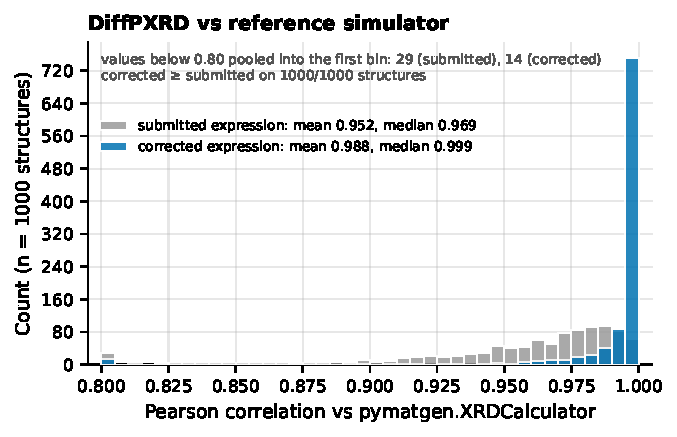
\includegraphics[keepaspectratio,alt={Figure 1. Differentiable-simulator validation. Distribution of Pearson correlation between the PyTorch DiffPXRD module and pymatgen.XRDCalculator over the first 1000 MP-20 test structures, with the corrected form factor (mean 0.988, median 0.999) and with the form factor of the submitted version (mean 0.952, median 0.969). The correction improves every structure. The residual lower tail is dominated by layered structures with strong texture in the reference.}]{fig3_diffpxrd_validation.pdf}}
\caption{\textbf{Figure 1. Differentiable-simulator validation.}
Distribution of Pearson correlation between the PyTorch DiffPXRD module
and \protect\texttt{pymatgen.XRDCalculator} over the first 1000 MP-20
test structures, with the corrected form factor (mean 0.988, median
0.999) and with the form factor of the submitted version (mean 0.952,
median 0.969). The correction improves every structure. The residual
lower tail is dominated by layered structures with strong texture in the
reference.}\label{fig:validation}
\end{figure}

\textbf{As a loss.} During training we recover an estimate
\(\hat{\mathbf{F}}\) of the clean coordinates from the model output (see
§3.4), simulate
\(\hat{\mathbf{p}} = \text{DiffPXRD}(\hat{\mathbf{F}}, \mathbf{Z}, \mathbf{L}_\text{true})\),
and compare with the input pattern via a Pearson-correlation loss
\(\mathcal{L}_\text{Debye} = 1 - \rho(\hat{\mathbf{p}}, \mathbf{p})\).
We use the true lattice for this auxiliary loss because the
differentiable simulator is more sensitive to lattice errors than to
coordinate errors at the early stages of training, and disentangling the
two signals proved more stable.

\subsection{3.4 Training objective}\label{training-objective}

We use a VP-SDE with cosine schedule (Nichol \& Dhariwal, 2021) for both
channels: \[
\bar{\alpha}(t) = \cos^2\!\left(\frac{\pi}{2} \cdot \frac{t + s}{1 + s}\right),\quad s = 0.008,\quad t \in [0,1].
\] Coordinates are diffused on the flat torus \(\mathbb{T}^3\) by
wrapping the noisy sample to \([0,1)^3\); the loss is computed on the
periodic difference
\((\hat{\mathbf{F}} - \mathbf{F} + 0.5) \bmod 1 - 0.5\). Lattice
parameters are diffused in \(\mathbb{R}^6\) after standardisation by the
train-set mean and standard deviation.

The full training objective (best configuration, run \texttt{gpu\_v13})
is \[
\mathcal{L} = \mathcal{L}_\text{coord} + \lambda_\text{lat}\,\mathcal{L}_\text{lat} + \lambda_\text{aux}\,\mathcal{L}_\text{aux} + \lambda_\text{Debye}\,\mathcal{L}_\text{Debye},
\] with \(\lambda_\text{lat} = 0.1\), \(\lambda_\text{aux} = 0.5\),
\(\lambda_\text{Debye} = 1.0\).

\textbf{Two non-trivial parameterisation choices.} Both are essential
and were arrived at by ablation, not foresight.

\emph{x₀-residual prediction.} Rather than asking the model to predict
noise \(\boldsymbol{\epsilon}\), the heads predict a \textbf{residual}
that is added to the noisy input to obtain the clean estimate: \[
\hat{\mathbf{F}}^{(0)} = \mathbf{F}^{(t)} + \text{Coord-Head}(\mathbf{h}),\quad
\hat{\boldsymbol{\ell}}^{(0)} = \boldsymbol{\ell}^{(t)} + \text{Lat-Head}(\cdot).
\] Because the heads are MLPs initialised to output near-zero, this
means the model starts as the identity transform: at \(t \approx 1\)
(near pure noise) the model outputs the noisy input as its
\(\hat{\mathbf{F}}^{(0)}\) estimate, which is wrong but at least
bounded; ε-prediction with the same architecture had to learn the entire
transform from random initialisation and never recovered. At single seed
this change appeared to lift the headline match metric 3.5×; a
multi-seed checkpoint sweep (§7) shows that match-rate lift does not
replicate, but the parameterisation does reproducibly improve the
pattern-Pearson (≈ 0.36 → 0.40, see §5.1).

\textbf{Correction made during review.} In x₀-residual mode the Debye
loss must be evaluated on the clean-coordinate estimate
\(\hat{\mathbf{F}}^{(0)} = \mathbf{F}^{(t)} + \text{Coord-Head}(\mathbf{h})\).
The submitted code evaluated it on the residual
\(\text{Coord-Head}(\mathbf{h})\) alone. For every x₀-residual run (v13,
v14, v15, v16 and the Phase 9 checkpoint v21) the Debye term therefore
compared the pattern of the wrong tensor with the target. The ε-mode
runs v10 and v11 were unaffected, as were the coordinate and lattice
losses and every evaluation-time number. The code is fixed. The affected
runs were retrained with the corrected loss and the corrected simulator
{[}PENDING C1: retrained numbers for the x₀-residual runs{]}.

\emph{Lattice-head input.} The lattice head reads the noisy lattice
\(\boldsymbol{\ell}^{(t)}\) as an explicit input feature. Without this,
i.e.~if the head only sees the (clean) lattice that is also passed to
the denoiser as the geometry context, the head can only ever predict the
unconditional mean noise, \(\mathbb{E}[\boldsymbol{\epsilon}] = 0\), and
its loss stays pinned at the random baseline of 1.0 forever. With this
fix, the lattice loss drops to 0.02--0.06 on stable runs.

We also experimented with two extensions that did not pan out (§5.4): a
\textbf{Wyckoff-site embedding} added to atom features, and an auxiliary
\textbf{distance-matrix loss} in which a pairwise MLP predicts
ground-truth periodic distances between atoms. Both are documented in
the released code behind the \texttt{-\/-use-wyckoff} and
\texttt{-\/-dist-weight} flags.

\subsection{3.5 Classical indexing as a control for the learned lattice
head}\label{classical-indexing-as-a-control-for-the-learned-lattice-head}

The lattice head described in §3.2 is the \emph{only} path by which the
model encodes absolute d-spacings: every Bragg reflection 2θ position is
set by the lattice through Bragg's law, so the lattice parameters are
the absolute reference frame against which all peak positions in the
input pattern must be interpreted. As §5.5 shows, the encoder + denoiser
learns \emph{relative} d-spacing structure (Pearson 0.43 between
predicted and target patterns at evaluation time, vs 0.97 between target
and ground truth) but not the absolute scale. Classical autoindexing,
which extracts peak positions, maps them to Q-space (Q = 4π sinθ/λ), and
fits a unit cell by enumeration of (h,k,l) → Q²(h,k,l), has solved this
sub-problem since the 1970s and runs on a CPU in milliseconds per
pattern.

We implement a from-scratch Q-space autoindexer that takes (i) the same
simulated PXRD pattern fed to the encoder and (ii) the true crystal
system of the target structure, supplied as a Bravais code, and returns
a candidate (a, b, c, α, β, γ). Item (ii) is prior information beyond
the composition that the learned head receives. It makes the indexer an
optimistic control rather than a fair competitor, and every indexer
number in this paper should be read with that in mind (see also §7 and
the unknown-system run below). Peak picking uses a 1D local-maximum
filter with a relative-intensity floor; the candidate Q-vector is fit by
least squares to the de-Wolff dichotomy parameter form for each Bravais
lattice. At sampling time we run the indexer first, substitute its
output for the lattice channel of the diffusion sampler, and run DDIM
only on the coordinate channel.

\textbf{Per-system accuracy (n = 1000 MP-20 test).} Native indexer
overall: 48.8 \% strict cell match, 1.45 Å mean cell-length MAE. Per
crystal system: hexagonal 77.9 \% / 0.53 Å, orthorhombic 59.8 \% / 0.96
Å, trigonal 43.3 \% / 4.62 Å, monoclinic 18.9 \% / 1.76 Å, triclinic 0
\%. The low-symmetry blowup (monoclinic and triclinic each have ≥ 4 free
cell parameters and the de-Wolff search becomes hypothesis-capped) is
the dominant remaining error. We ship a GSAS-II (Toby \& Von Dreele,
2013) adapter (\texttt{src/pxrd\_diff/indexer\_gsas.py}) for the
low-symmetry path behind a \texttt{-\/-use-gsas} opt-in flag; in
practice \texttt{DoIndexPeaks} hangs on real MP-20 monoclinic/triclinic
patterns inside \texttt{findBestCell} and is documented experimental
rather than headline.

\textbf{Without the crystal system.} At a referee's request the indexer
was also run with no crystal system supplied. Cubic, tetragonal,
hexagonal/trigonal, orthorhombic and monoclinic cells are all searched,
and the candidate with the highest de-Wolff M20 figure of merit is kept.
{[}PENDING B2: per-system strict \% and length MAE, and the fraction of
patterns whose lattice type is recovered, on the same n = 1000.{]}
{[}PENDING C3: downstream match rate at three seeds when these cells
replace the learned head.{]}

The indexer is a drop-in in the mechanical sense: training is unchanged,
and the diffusion sampler is unchanged except for the lattice-channel
substitution at t = T. Patterns for which the indexer returns no cell
(39 of the 1000 test patterns) are scored as misses. The submitted
version had given them the true lattice; §5.7 reports the correction and
its effect. The headline metric (§5.2) reports both with and without the
indexer for direct comparison.

\subsection{3.6 Sampling}\label{sampling}

DDIM (Song \emph{et al.}, 2021) with 50 steps and \(\eta = 0\). We start
from independent standard Gaussian noise on the lattice and on the
(un-wrapped) coordinates, then alternate the standard DDIM update on
each channel. Coordinates are wrapped to \([0,1)\) after every step.
Predicted lattice parameters are de-standardised at the end and clipped
to physically valid ranges \((a,b,c) \in [0.5, 100]\) Å,
\((\alpha,\beta,\gamma) \in [10°, 170°]\) before being passed to
\texttt{pymatgen.Lattice.from\_parameters}.

A subtle bug fix is worth noting. In the x₀-residual variant, recovering
the implicit ε for the DDIM update requires dividing by
\(\sqrt{1-\bar{\alpha}(t)}\); near \(t = 0\) this denominator vanishes.
We clamp it to 0.05 and skip the very last DDIM step when sampling,
which removed a class of structures with NaN coordinates that we
initially saw.

\begin{center}\rule{0.5\linewidth}{0.5pt}\end{center}

\section{4. Experiments}\label{experiments}

\textbf{Dataset.} Canonical CDVAE (Xie \emph{et al.}, 2022) MP-20 split:
27 136 / 9 047 / 9 046 train/val/test, ≤ 20 atoms/conventional cell.
Patterns simulated with \texttt{pymatgen.XRDCalculator} (Cu Kα₁, λ =
1.54184 Å), max-normalised, 4 251 bins 5--90° / 0.02°; cached as
\texttt{.npz}, zero failures over 45 196 structures.

\textbf{Evaluation.} Three views: (1) \textbf{composition match}
(trivial, \(\mathbf{Z}\) given); (2) \textbf{structure match} via
\texttt{pymatgen.StructureMatcher} at
\((\ell_\text{tol}, s_\text{tol}, \alpha_\text{tol}) = (0.2, 0.3, 5°)\),
the headline ``match rate''; (3) \textbf{coordinate RMSD} on aligned,
permuted atoms when matched. We also report space-group match at symprec
\(\in \{0.01, 0.05, 0.1, 0.2\}\), pattern Pearson, and \(R_{wp}\).

The stricter \textbf{``all-correct''} rule combines
\texttt{composition\ ∧\ sg-match@symprec=0.1\ ∧\ rmsd\ ≤\ 0.1\ Å}, the
experimentally relevant case for downstream crystallographic use.

Two evaluation modes: \emph{full pipeline} (predicted lattice + coords)
and \emph{true-lattice/coord-only} (ground-truth lattice substituted).
The latter isolates coordinate quality from lattice quality and is the
stricter ablation setting. In the indexer mode (§3.5) a pattern the
indexer cannot index counts as a miss; it is never scored with the true
lattice.

\textbf{Implementation.} AdamW, learning rate \(10^{-3}\) (the value
stored in the released v21 checkpoint; the submitted text gave
\(5\times10^{-4}\), see §5.7(d)), cosine decay to zero over 100 k steps,
WD \(10^{-4}\), grad-clip 1.0. Batch 64, \textasciitilde24 epochs,
single RTX 5090 (\textasciitilde1.5--1.7 h/run). 3.7 M parameters;
\(L=5, d=384\) (\textasciitilde10 M) gave no benefit (§5.2). VP-SDE with
\(t \sim U(0,1)\). Total compute: \textasciitilde35 GPU-hours,
\textasciitilde USD 25 on Vast.ai (Phase 4 ablation + Phase 9 v21
retrain + indexer/perturbation sweeps + DGpt n=1000 + PXRDnet n=20 +
evaluation).

\begin{center}\rule{0.5\linewidth}{0.5pt}\end{center}

\section{5. Results}\label{results}

Order: Phase 4 architectural ablation (§5.1) → Phase 9 indexer drop-in
(§5.2) → reproduced baselines (§5.3) → failure catalogue (§5.4) →
encoder-bottleneck perturbation study (§5.5).

\subsection{5.1 Phase 4: architectural ablation (true-lattice
setting)}\label{phase-4-architectural-ablation-true-lattice-setting}

Table 1: seven runs sweeping the Debye loss, the lattice-input fix,
x₀-residual, and two extensions (Wyckoff, distance loss), all on n = 1
000 MP-20 test with true lattice substituted. Every row is a single
training seed. The table is exploratory: it guided the design, and only
the ε-vs-x₀-residual contrast was later replicated across seeds (§7).
Runs v11 and v13--v16 were trained with the submitted version's
simulator, and v13--v16 with the x₀-mode Debye defect (§3.3, §3.4)
{[}PENDING C1: retrained rows, or a statement of which rows were
retrained{]}.

\textbf{Table 1.} Phase 4 coordinate-only ablation, MP-20 test (n = 1
000, true lattice substituted). Single seed per row; exploratory.

{\def\LTcaptype{none} % do not increment counter
\begin{longtable}[]{@{}
  >{\raggedright\arraybackslash}p{(\linewidth - 14\tabcolsep) * \real{0.0886}}
  >{\raggedright\arraybackslash}p{(\linewidth - 14\tabcolsep) * \real{0.2278}}
  >{\raggedright\arraybackslash}p{(\linewidth - 14\tabcolsep) * \real{0.1139}}
  >{\raggedright\arraybackslash}p{(\linewidth - 14\tabcolsep) * \real{0.1139}}
  >{\raggedright\arraybackslash}p{(\linewidth - 14\tabcolsep) * \real{0.1013}}
  >{\raggedright\arraybackslash}p{(\linewidth - 14\tabcolsep) * \real{0.1139}}
  >{\raggedright\arraybackslash}p{(\linewidth - 14\tabcolsep) * \real{0.1139}}
  >{\raggedright\arraybackslash}p{(\linewidth - 14\tabcolsep) * \real{0.1266}}@{}}
\toprule\noalign{}
\begin{minipage}[b]{\linewidth}\raggedright
Run
\end{minipage} & \begin{minipage}[b]{\linewidth}\raggedright
Parameterisation
\end{minipage} & \begin{minipage}[b]{\linewidth}\raggedright
λ\_Debye
\end{minipage} & \begin{minipage}[b]{\linewidth}\raggedright
Wyckoff
\end{minipage} & \begin{minipage}[b]{\linewidth}\raggedright
λ\_dist
\end{minipage} & \begin{minipage}[b]{\linewidth}\raggedright
Match \%
\end{minipage} & \begin{minipage}[b]{\linewidth}\raggedright
Pearson
\end{minipage} & \begin{minipage}[b]{\linewidth}\raggedright
RMSD (Å)
\end{minipage} \\
\midrule\noalign{}
\endhead
\bottomrule\noalign{}
\endlastfoot
v10 & ε & 0 & -- & 0 & 1.40 & 0.359 & 0.17 \\
v11 & ε & 1 & -- & 0 & 0.90 & 0.365 & 0.15 \\
\textbf{v13} & \textbf{x₀-residual} & \textbf{1} & \textbf{--} &
\textbf{0} & \textbf{2.51} & \textbf{0.434} & 0.22 \\
v14 & x₀-residual & 1 & yes & 0.01 & 0.80 & 0.367 & 0.14 \\
v15 & x₀-residual & 1 & yes & 0 & 2.10 & 0.392 & 0.21 \\
v16 & x₀-residual & 1 & -- & 0.01 & 1.80 & 0.368 & 0.22 \\
\end{longtable}
}

\begin{figure}
\centering
\pandocbounded{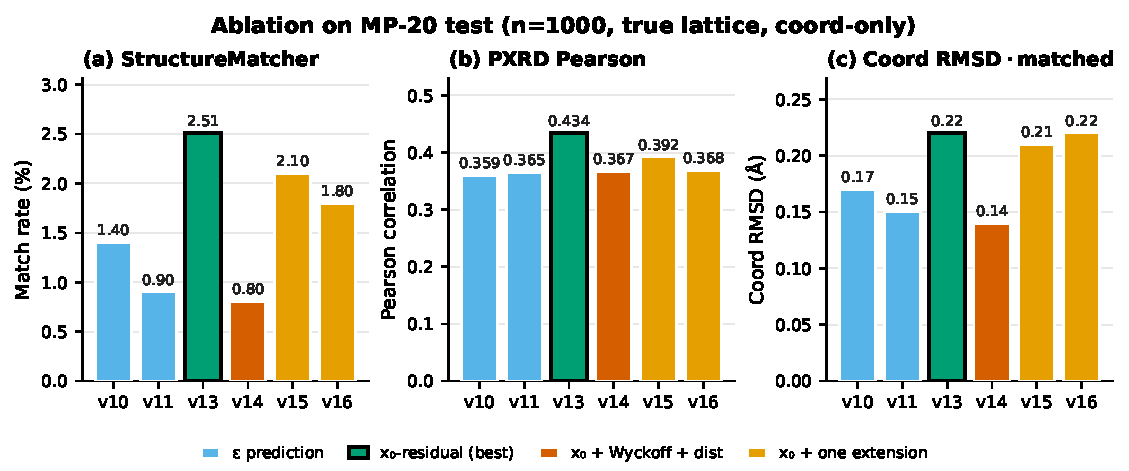
\includegraphics[keepaspectratio,alt={Figure 2. Phase 4 architectural ablation (single seed per run; exploratory). Match rate (a) and pattern Pearson (b) for the seven coordinate-only runs of Table 1 on MP-20 test (n = 1000, true lattice substituted). The ε → x₀-residual switch (v11 → v13) shows the largest single-seed match lift (panel a), but that match lift does not replicate across seeds; only the pattern-Pearson gain (panel b) does (§7); adding Wyckoff embeddings or a distance-matrix loss regresses below it.}]{fig1_ablation.pdf}}
\caption{\textbf{Figure 2. Phase 4 architectural ablation (single seed
per run; exploratory).} Match rate (a) and pattern Pearson (b) for the
seven coordinate-only runs of Table 1 on MP-20 test (n = 1000, true
lattice substituted). The ε → x₀-residual switch (v11 → v13) shows the
largest single-seed match lift (panel a), but that match lift does not
replicate across seeds; only the pattern-Pearson gain (panel b) does
(§7); adding Wyckoff embeddings or a distance-matrix loss regresses
below it.}\label{fig:ablation}
\end{figure}

The \textbf{lattice-input fix} (§3.4) is load-bearing: it drops lattice
loss from 1.0 (pinned at the prior variance for 100 k steps) to
\textasciitilde0.02 once \(W_\text{lat}\boldsymbol{\ell}^{(t)}\) enters
the head input. A second, apparent lift did \textbf{not} survive
replication: switching from \textbf{ε to x₀-residual} at fixed Debye λ =
1 (v11 → v13) lifted single-seed match 0.9 \% → 2.5 \%, but a multi-seed
checkpoint sweep (two seeds × five checkpoints, 20k--100k) found ε and
x₀-residual indistinguishable on match rate (1.20 \% vs 1.35 \% pooled;
x₀ never exceeds 1.5 \% at any checkpoint, including the 80 k one
matching the original's 79.5 k, §7), so the 3.5× match lift was a
single-seed fluctuation. The x₀-residual parameterisation does, however,
reproducibly improve pattern-Pearson (0.36 → 0.40), which is the part of
the Phase-4 signal that survives. Capacity is not the bottleneck: a 10.1
M-parameter run (\(d=384\), \(L=5\), \texttt{gpu\_v12}) stayed at the
same \textasciitilde1.0 coord-loss plateau as v10. Under the full
pipeline (sampled lattice), v13 drops to 1.2 \% at n = 256; the Phase 9
v21 checkpoint reaches 4.5 \% under oracle (three seeds; an earlier
single-seed snapshot read 5.6 \%) but only 1.0 \% under full pipeline.
§5.2 attacks that gap.

\subsection{5.2 Phase 9: classical indexer
control}\label{phase-9-classical-indexer-control}

Table 2: three rows on the same n = 1 000 with the v21 checkpoint (Phase
9 retrain, Phase 4 fixes + retuned encoder); they differ only in which
lattice the sampler conditions on. The indexer row is a control with
extra prior information: the indexer is supplied with the true crystal
system (§3.5).

\textbf{Table 2.} Phase 9 lattice-source comparison (n = 1 000 MP-20
test, v21 checkpoint, single-seed snapshot). The indexer receives the
true crystal system. Match \% with 95 \% Wilson CI; the three-seed
paired analysis follows below. {[}PENDING C1: replace with the
retrained-v21 snapshot if the retrain changes these rows.{]}

{\def\LTcaptype{none} % do not increment counter
\begin{longtable}[]{@{}
  >{\raggedright\arraybackslash}p{(\linewidth - 10\tabcolsep) * \real{0.4234}}
  >{\raggedright\arraybackslash}p{(\linewidth - 10\tabcolsep) * \real{0.1712}}
  >{\raggedright\arraybackslash}p{(\linewidth - 10\tabcolsep) * \real{0.1351}}
  >{\raggedright\arraybackslash}p{(\linewidth - 10\tabcolsep) * \real{0.0901}}
  >{\raggedright\arraybackslash}p{(\linewidth - 10\tabcolsep) * \real{0.1261}}
  >{\raggedright\arraybackslash}p{(\linewidth - 10\tabcolsep) * \real{0.0541}}@{}}
\toprule\noalign{}
\begin{minipage}[b]{\linewidth}\raggedright
Lattice source
\end{minipage} & \begin{minipage}[b]{\linewidth}\raggedright
Match \% (95 \% CI)
\end{minipage} & \begin{minipage}[b]{\linewidth}\raggedright
All-correct \%
\end{minipage} & \begin{minipage}[b]{\linewidth}\raggedright
sg@0.1 \%
\end{minipage} & \begin{minipage}[b]{\linewidth}\raggedright
RMSD med (Å)
\end{minipage} & \begin{minipage}[b]{\linewidth}\raggedright
R\_wp
\end{minipage} \\
\midrule\noalign{}
\endhead
\bottomrule\noalign{}
\endlastfoot
Learned head only (full pipeline) & 1.0 {[}0.5, 1.8{]} & 0.0 & 1.4 & n/a
& 11.7 \\
\textbf{Classical Q-space autoindexer (§3.5), crystal system given} &
\textbf{1.6 {[}1.0, 2.6{]}} & \textbf{0.1} & \textbf{1.4} &
\textbf{0.125} & 11.5 \\
Ground-truth lattice (oracle) & 5.6 {[}4.3, 7.2{]} & 0.6 & 1.7 & 0.106 &
5.6 \\
\end{longtable}
}

\textbf{The lift is real: a three-seed paired test.} The single-seed
snapshot alone does not establish a genuine improvement: its Wilson CIs
overlap and an unpaired two-proportion test gives p = 0.24. To resolve
it we reran \emph{both} lattice sources at three seeds (n = 1 000 each),
differing only in the lattice channel, and applied a paired McNemar test
on the per-structure outcomes, the correct test, because the two arms
see the same materials. The result is unambiguous. The two arms are
scored on the same materials per seed, but the learned-head arm yields
fewer \emph{evaluable} cells: its diffusion-sampled lattices are
frequently degenerate and hang \texttt{StructureMatcher}/\texttt{spglib}
(C calls that a Python signal cannot interrupt), so we run
structure-domain scoring in a spawn worker hard-killed at 30 s and count
overruns as misses. This leaves \textbf{1 949} learned-head structures
scored across the three seeds. The indexer arm scores 2 883
structure-seeds: 39 patterns per seed, 117 in total, could not be
indexed and are counted as misses (the submitted version had given them
the true lattice; none of them matched under it, §5.7). The paired test
runs on the 1 949-structure intersection (every learned-head row has a
matched indexer row); 86 of these are unindexed patterns, which enter as
concordant misses and do not affect the discordant cells. On that paired
set the indexer recovers \textbf{27} structures the learned head misses
and the learned head recovers \textbf{none} the indexer misses (the
explicit 2×2 below).

\textbf{Table 2a.} Paired per-structure outcomes, learned head vs
indexer drop-in (three seeds pooled; match = \texttt{StructureMatcher}
hit).

{\def\LTcaptype{none} % do not increment counter
\begin{longtable}[]{@{}llll@{}}
\toprule\noalign{}
& indexer \textbf{match} & indexer \textbf{miss} & row total \\
\midrule\noalign{}
\endhead
\bottomrule\noalign{}
\endlastfoot
\textbf{learned match} & 0 & 0 & 0 \\
\textbf{learned miss} & 27 & 1 922 & 1 949 \\
\textbf{col total} & 27 & 1 922 & 1 949 \\
\end{longtable}
}

The discordant cells are \emph{b} = 27 (indexer fixes), \emph{c} = 0
(indexer breaks); an exact two-sided McNemar test gives \textbf{p = 1.5
× 10⁻⁸}. (Marginal match counts differ: indexer 46 / 2 883, learned 0 /
1 949, because 19 further indexer matches fall on structures the learned
arm could not score; these do not enter the paired test.) The
single-seed 1.0 \% learned-head figure in Table 2 is within run-to-run
noise of zero; across three fresh seeds the learned lattice head matched
nothing. The gain does \textbf{not} carry to the stricter all-correct
metric: there the discordant cells are \emph{b} = 4, \emph{c} = 0 (exact
McNemar \textbf{p = 0.13}): the indexer fixes the cell but not the space
group. So the control reproducibly improves match rate over the learned
lattice head. This is the expected outcome for a classical algorithm
handed the crystal system, and we read it as a sanity check on the
diagnosis rather than as a result about PXRD inversion. The
\emph{mechanism} (§5.5, §5.6) is that its gains come entirely from
high-symmetry systems where the indexer's cell error falls below the 0.5
Å sensitivity knee, with low-symmetry contributing nothing.

What the indexer does \emph{not} do is close the gap to the oracle. We
re-ran the oracle at three seeds, firming the single-seed 5.6 \% to
\textbf{4.5 \% {[}3.8, 5.3{]}} (135 / 3 000 pooled), still disjoint from
the indexer's 1.6 \% {[}1.2, 2.1{]}. The indexer → oracle gap (1.6 → 4.5
\%) is itself significant (disjoint CIs) and isolates the
lattice-attributable error: even with a perfect lattice, match caps at
4.5 \%, so coordinate prediction is the dominant limiter while lattice
error explains the 1.6 → 4.5 \% shortfall. The indexer's per-system MAE
(1.45 Å overall, dominated by mono 1.76 Å and triclinic NaN) sits above
the 0.5 Å knee; closing the rest requires fixing the low-symmetry path
(GSAS-II remains experimental).

\begin{figure}
\centering
\pandocbounded{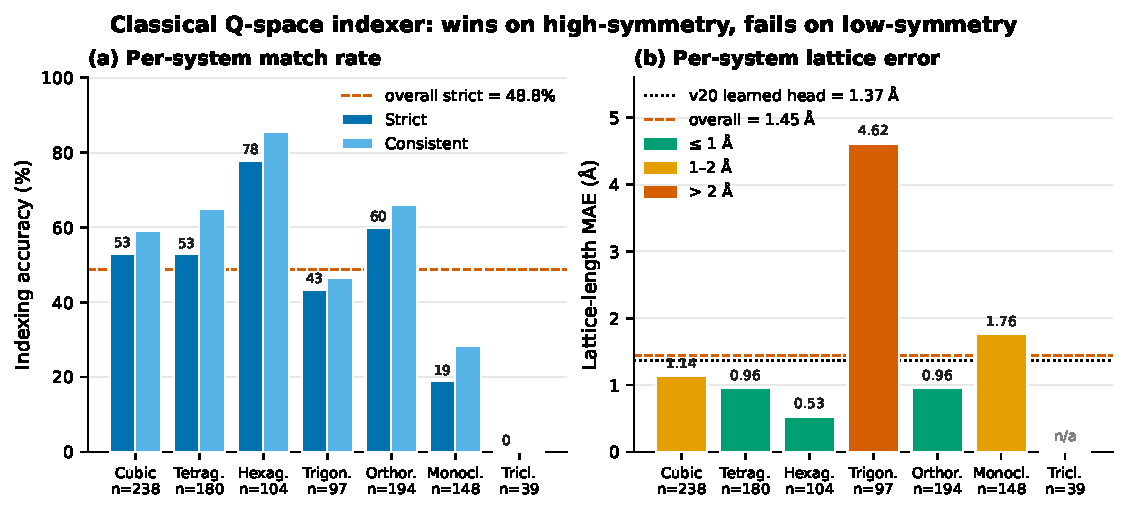
\includegraphics[keepaspectratio,alt={Figure 3. Per-system indexer performance. Strict and consistent indexing rates (a) and length MAE (b) on n = 1 000. High-symmetry systems (hex, ortho) sit below the 0.5 Å knee; trig and mono blow up; triclinic is unindexable in this implementation. The overall 1.45 Å MAE hides two regimes, and explains why the indexer's significant match-rate gain (§5.2) is concentrated entirely in the high-symmetry systems.}]{fig4_indexer_bench.pdf}}
\caption{\textbf{Figure 3. Per-system indexer performance.} Strict and
consistent indexing rates (a) and length MAE (b) on n = 1 000.
High-symmetry systems (hex, ortho) sit below the 0.5 Å knee; trig and
mono blow up; triclinic is unindexable in this implementation. The
overall 1.45 Å MAE hides two regimes, and explains why the indexer's
significant match-rate gain (§5.2) is concentrated entirely in the
high-symmetry systems.}\label{fig:indexer}
\end{figure}

\subsection{5.3 Head-to-head with external
baselines}\label{head-to-head-with-external-baselines}

DiffractGPT (\texttt{knc6/diffractgpt\_mistral\_chemical\_formula}) at n
= 1 000, PXRDnet (\texttt{therealgabeguo/cdvae\_xrd\_sinc100}) at n = 20
(limited by \textasciitilde4 GPU-hr/material), and deCIFer (deCIFer\_v1,
conditioned on XRD + composition) at n = 300 re-scored on \emph{our}
\texttt{StructureMatcher} harness at matching tolerances. Crystalyze's
checkpoint download is inactive; cite-but-not-reproduced.

\textbf{Table 3.} Reproduced head-to-head on MP-20 test
(StructureMatcher ltol 0.2, stol 0.3, angle\_tol 5°). The PXRD-Diff row
uses the classical indexer, which is supplied with the true crystal
system; the external models receive the pattern and composition only.
The rows set the scale of the diagnostic model and are not a
competitiveness claim.

{\def\LTcaptype{none} % do not increment counter
\begin{longtable}[]{@{}
  >{\raggedright\arraybackslash}p{(\linewidth - 10\tabcolsep) * \real{0.3770}}
  >{\raggedright\arraybackslash}p{(\linewidth - 10\tabcolsep) * \real{0.0574}}
  >{\raggedright\arraybackslash}p{(\linewidth - 10\tabcolsep) * \real{0.1639}}
  >{\raggedright\arraybackslash}p{(\linewidth - 10\tabcolsep) * \real{0.2049}}
  >{\raggedright\arraybackslash}p{(\linewidth - 10\tabcolsep) * \real{0.0820}}
  >{\raggedright\arraybackslash}p{(\linewidth - 10\tabcolsep) * \real{0.1148}}@{}}
\toprule\noalign{}
\begin{minipage}[b]{\linewidth}\raggedright
Model
\end{minipage} & \begin{minipage}[b]{\linewidth}\raggedright
n
\end{minipage} & \begin{minipage}[b]{\linewidth}\raggedright
Match \% (95 \% CI)
\end{minipage} & \begin{minipage}[b]{\linewidth}\raggedright
All-correct \% (95 \% CI)
\end{minipage} & \begin{minipage}[b]{\linewidth}\raggedright
sg@0.1 \%
\end{minipage} & \begin{minipage}[b]{\linewidth}\raggedright
RMSD med (Å)
\end{minipage} \\
\midrule\noalign{}
\endhead
\bottomrule\noalign{}
\endlastfoot
PXRD-Diff (v21 + indexer control, crystal system given) & 1 000 & 1.6
{[}1.0, 2.6{]} & 0.1 {[}0.0, 0.6{]} & 1.4 & 0.125 \\
DiffractGPT (Choudhary, 2025) & 1 000 & 18.9 {[}16.6, 21.4{]} & 15.9
{[}13.8, 18.3{]} & 21.3 & 0.001 \\
PXRDnet sinc100 (Guo \emph{et al.}, 2025) & 20 & 30.0 {[}14.5, 51.9{]} &
5.0 {[}0.9, 23.6{]} & 5.0 & 0.011 \\
deCIFer (Johansen \emph{et al.}, 2025) & 298 & 73.8 {[}68.6, 78.5{]} &
69.5 {[}64.0, 74.4{]} & 83.6 & 0.009 \\
\end{longtable}
}

\textbf{Match rate} ranks deCIFer ≫ PXRDnet \textgreater{} DGpt
\textgreater{} PXRD-Diff. deCIFer, a concurrent autoregressive CIF-token
model conditioned on XRD + composition, is the strongest external
reference at 73.8 \% match / 69.5 \% all-correct (n = 300). Its
all-correct nearly equals its match: when it recovers structure it
almost always recovers the space group too, the same CIF-token signature
seen in DGpt. PXRDnet's lead over DGpt is consistent with its 35 k-op
latent optimisation, whereas DGpt is one forward pass. PXRD-Diff, at 1.6
\%, sits an order of magnitude below all three, as expected for a 3.7
M-parameter diagnostic model. A more interesting pattern is that the
\emph{all-correct} ordering need not follow match rate: DGpt's
all-correct (15.9 \% {[}13.8, 18.3{]}) exceeds its space-group-loose
match by little, while PXRDnet's drops from 30 \% match to 5 \%
all-correct, i.e.~PXRDnet matches structure under loose tolerances but
rarely recovers the space group, whereas DGpt's CIF-token output appears
to encode symmetry. \textbf{We flag this as a hypothesis, not a
finding.} At n = 20 the PXRDnet all-correct estimate (1/20) carries a 95
\% CI of {[}0.9, 23.6{]}, which overlaps DGpt's {[}13.8, 18.3{]}; the
apparent ``reversal'' is \emph{not} statistically established and would
require n ≈ 100--200 to confirm. If it holds, the implication is
consequential: published single-number ``match rates'' would conflate
structure recovery with symmetry recovery, which is precisely why we
surface it despite the underpowered sample, and why §6 frames it as
motivation for future measurement rather than a claim. \textbf{RMSD} is
heavy-tailed for us and tight-near-zero for both baselines, suggesting
our matches are tolerance-stretch rather than coordinate recovery.

\textbf{What the gap does and does not reflect.} All four systems are
given the composition (§3.1). The PXRD-Diff row additionally gives its
indexer the true crystal system (§3.5), so on prior information
PXRD-Diff is favoured, not handicapped. On the pattern itself the
asymmetry runs the other way. DiffractGPT is conditioned on a
\textbf{coarse 300-bin pattern} (2θ ∈ {[}0, 90°{]}, 0.3° bins, rendered
as a \texttt{;}-separated string), an order of magnitude lower
resolution than PXRD-Diff's 4 251-bin 0.02° input, yet it still reaches
18.9 \%. So the external models do not win by seeing more of the
pattern. The differences that matter are \textbf{capacity} (DiffractGPT
is a 7 B-parameter LLM; PXRD-Diff is 3.7 M, three orders of magnitude)
and \textbf{inference compute} (PXRDnet's \textasciitilde35 k-op latent
optimisation vs our single DDIM pass). Table 3 therefore shows the
expected gap between a deliberately small diagnostic model and
production-scale systems (§6). It is reported to set the scale, not to
rank PXRD-Diff among them.

\begin{figure}
\centering
\pandocbounded{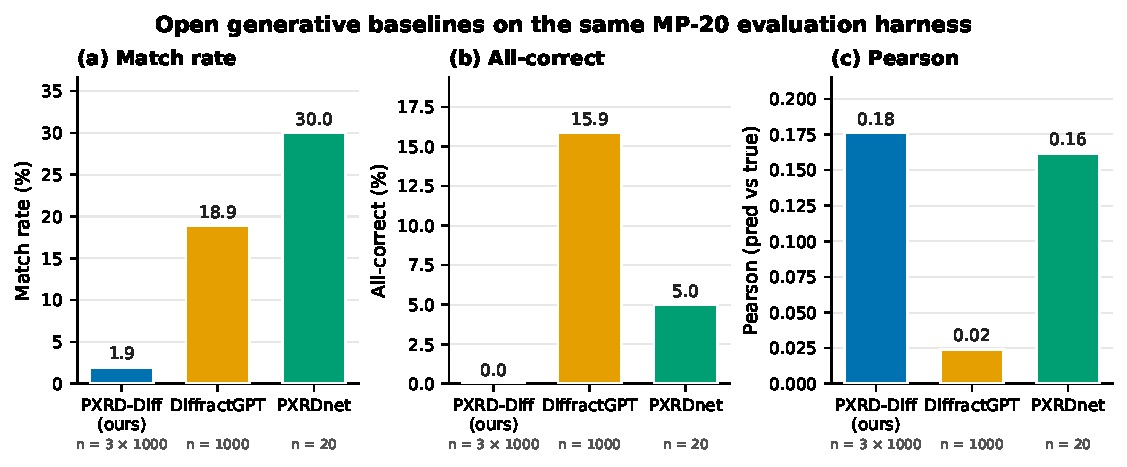
\includegraphics[keepaspectratio,alt={Figure 4. Three-way headline comparison. Match rate, all-correct, and pattern-Pearson on the same MP-20 test materials scored through our StructureMatcher harness, with 95 \% Wilson CIs. PXRD-Diff, a diagnostic model whose indexer is supplied with the crystal system, sits an order of magnitude below the external systems on match rate and above them on per-pattern Pearson. Note the wide PXRDnet (n = 20) intervals: the DGpt \textgreater{} PXRDnet all-correct ordering is a hypothesis, not an established result (§5.3, §6).}]{fig5_threeway_headline.pdf}}
\caption{\textbf{Figure 4. Three-way headline comparison.} Match rate,
all-correct, and pattern-Pearson on the same MP-20 test materials scored
through \emph{our} \protect\texttt{StructureMatcher} harness, with 95 \%
Wilson CIs. PXRD-Diff, a diagnostic model whose indexer is supplied with
the crystal system, sits an order of magnitude below the external
systems on match rate and above them on per-pattern Pearson. Note the
wide PXRDnet (n = 20) intervals: the DGpt \textgreater{} PXRDnet
all-correct ordering is a hypothesis, not an established result (§5.3,
§6).}\label{fig:threeway}
\end{figure}

\emph{Caveats.} PXRDnet n = 20 has a 95 \% Wilson CI of roughly ±20 pp
on every rate; n = 200 would need \textasciitilde33 days of RTX 5090
rental at \textasciitilde4 GPU-hr/material. Patterns are simulated
through each model's own preprocessing (different bins, 2θ vs Q,
broadening): material\_ids are identical, pattern inputs are not
bit-identical; §7 bounds this.

\subsection{\texorpdfstring{5.4 What did \emph{not}
work}{5.4 What did not work}}\label{what-did-not-work}

Four interventions failed at n ≥ 200; one paragraph each.

\textbf{Top-K Debye rerank (Phase 9.1.4).} Top-5 indexer candidates
reranked by Debye loss: match 1.6 \% → 1.0 \%, all-correct 0.1 \% → 0.0
\% at n = 1 000. The indexer surfaces more wrong cells faster than
rerank can filter.

\textbf{Debye-gradient guidance during DDIM (Phase 9.2).}
Coordinate-channel guidance term
\(-g \cdot \nabla_{\mathcal{C}} \mathcal{L}_\text{Debye}\), sweep
\(g \in \{0,0.5,1,2,5\}\) on n = 200: flat 1.0--2.5 \% within noise,
all-correct 0 \% throughout. Sampling-time Debye gradient is too noisy
to steer the trajectory, consistent with Segal \emph{et al.} (2026), who
show the powder-XRD similarity loss landscape is too non-convex for
direct gradient descent.

\textbf{Wyckoff-letter embeddings (v15, n = 1 000).} Each atom received
an \texttt{nn.Embedding(27,\ 256)} token for its
\texttt{spglib}-assigned Wyckoff letter. A Wyckoff letter is meaningful
only within a given space group: the same letter denotes different
multiplicities, site symmetries and coordinate constraints in different
groups (Dauter \& Jaskolski, 2010; de la Flor \emph{et al.}, 2023). The
embedding therefore carried a label, not a constraint. Atomic
coordinates were still generated freely, and nothing in the loss or the
sampler enforced the fixed or symmetry-related coordinates that a
Wyckoff position implies. The embedding learns (5 404 of 6 912 entries
non-zero), but match drops from 2.5 \% to 2.1 \% and lattice prediction
destabilises (lattice loss \textasciitilde0.6 vs \textasciitilde0.02;
Figure 5). We suspect the inflated atom-feature norm shifts the
lattice-pool input distribution. The negative result is narrow. It shows
that a space-group-agnostic label token does not help and may hurt
training dynamics. It says nothing about whether symmetry information
imposed as a constraint, on the coordinates or on the space group, would
help; that experiment was not run.

\begin{figure}
\centering
\pandocbounded{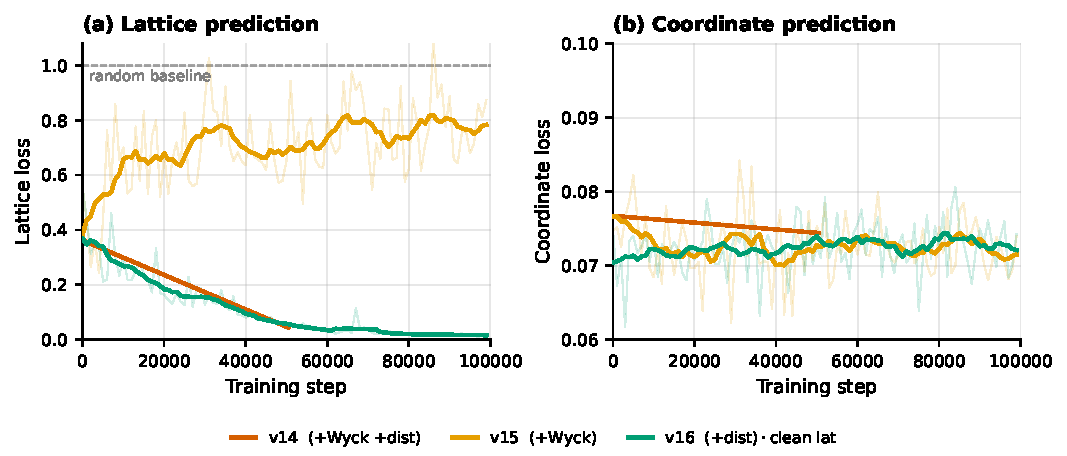
\includegraphics[keepaspectratio,alt={Figure 5. Wyckoff embedding destabilises lattice prediction. Lattice (a) and coordinate (b) training-loss curves for the distance-aux run (v16) vs the Wyckoff-embedding run (v15). Adding the Wyckoff embedding inflates the lattice loss by an order of magnitude (\textasciitilde0.6 vs \textasciitilde0.02) while leaving the coordinate loss largely unchanged; the failure is localised to the lattice channel.}]{fig2_training_curves.pdf}}
\caption{\textbf{Figure 5. Wyckoff embedding destabilises lattice
prediction.} Lattice (a) and coordinate (b) training-loss curves for the
distance-aux run (v16) vs the Wyckoff-embedding run (v15). Adding the
Wyckoff embedding inflates the lattice loss by an order of magnitude
(\textasciitilde0.6 vs \textasciitilde0.02) while leaving the coordinate
loss largely unchanged; the failure is localised to the lattice
channel.}\label{fig:training}
\end{figure}

\textbf{Distance-matrix aux loss (v16, n = 1 000).} Pairwise MLP
predicting periodic distances, \(\lambda_\text{dist} = 0.01\) (largest
stable). Loss decreases (final \textasciitilde2.0 vs \textasciitilde10
random) but match drops 2.5 \% → 1.8 \%; biases features toward
absolute-distance reconstruction rather than the relative updates
diffusion needs.

\textbf{Combination (v14).} Wyckoff + distance loss together collapses
to 0.8 \%, below the bare ε baseline; the two interact destructively, no
clean theoretical explanation.

\subsection{5.5 Encoder-bottleneck perturbation
study}\label{encoder-bottleneck-perturbation-study}

Best predicted-vs-target Pearson is 0.43; the same model with
\emph{correct} coordinates plugged into the differentiable simulator
hits 0.97; the encoder + denoiser leaves \textasciitilde0.5 of
pattern-space agreement on the table. The aux head (sees \(\mathbf{g}\)
only) reaches a 0.007 \emph{normalised} lattice-regression loss, but
that figure is a relative fit that does \textbf{not} survive conversion
to absolute scale: when the aux head's own lattice is substituted into
the sampler it recovers only 1.2 \% (§5.6), because its 1.1 Å length MAE
shifts every Bragg reflection by \textasciitilde15 \%. So the global
encoding carries crystal-system and relative-spacing structure but not
absolute d-spacings at the \textless0.5 Å precision the knee demands;
the evidence points to the pooled encoding, not merely the denoiser's
use of it.

Perturbing the sampler-supplied lattice by Å of cell-length error, v21
at n = 200: match decays 5.6 \% (Δ=0) → 2.0 \% (0.5 Å) → 0.5 \% (1.0 Å)
→ 0 \% (≥1.5 Å), steeper than linear with a knee at \textasciitilde0.5
Å. This matches the indexer's per-system MAE: high-symmetry systems
(hex, ortho; MAE ≤ 1.0 Å) lift; low-symmetry (mono, tri; MAE ≥ 1.5 Å) do
not. §5.2's indexer lift is \emph{predictable}: it works where it can.

\subsection{5.6 Why the learned lattice fails: a pooling bottleneck, not
a head
bottleneck}\label{why-the-learned-lattice-fails-a-pooling-bottleneck-not-a-head-bottleneck}

The natural reading of the 0.007 aux loss, that the lattice is already
recoverable from the encoder and only the denoiser is at fault, is
testable, and it is wrong. Two experiments (released as
\texttt{paper/phase5\_results/} and \texttt{paper/phase5b6\_results/})
promote the auxiliary head from a training-time regulariser to the
inference-time lattice source and measure what it actually delivers.

\textbf{Aux head as lattice predictor (no retrain).} Substituting the
v13 aux head's predicted \((a,b,c,\alpha,\beta,\gamma)\) for the sampled
lattice channel at n = 1 000 gives a length MAE of (1.12, 1.02, 1.38) Å
and an angle MAE of (13.0°, 11.9°, 17.6°) at \textbf{99.8 \%} cell
validity, far better conditioned than the diffusion sampler, whose
predicted cells are near-0 \% valid, but still \textasciitilde15 \%
relative length error. End-to-end this recovers \textbf{1.2 \%} match
(1.3 \% with Phase 4 ensembling + coordinate refinement) and 0.0 \%
all-correct, with pattern Pearson collapsing to \textbf{0.013}: a 15 \%
length error shifts every Bragg reflection by a similar fraction in 2θ,
so the simulated pattern no longer overlaps the target.

\textbf{Stronger, constrained supervision (retrain).} Bounding the head
(softplus lengths, sigmoid-scaled angles), raising the aux weight 0.5 →
5.0, and warm-starting 30 k further steps leaves the MAE essentially
unchanged (a ≈ 1.11 Å, α ≈ 14°). The error behaves like a property of
the \emph{pooled global encoding} rather than of the head: the
\texttt{AdaptiveAvgPool1d(1)} collapse that §3.2 already identified for
coordinates would discard the peak-position fidelity Bragg's-law
decoding needs to fix absolute lengths, and no head reading
\(\mathbf{g}\) recovers it. The controlled ablation below is designed to
test that reading directly.

This reconciles the diagnosis with the indexer result. The 0.007
normalised aux loss is a \emph{relative} fit, enough to place the
crystal system (a space-group head on the same encoder reaches 39 \%
top-1 / 71 \% top-5 across 230 classes, released under
\texttt{phase5b6\_results/}) but not the absolute scale. The classical
autoindexer succeeds exactly where the encoder fails because it reads
peak \emph{positions} directly rather than a pooled summary; this is why
§5.2's lift lives entirely in the high-symmetry systems where peak
positions over-determine the cell, and why head-side fixes (Phase 5
here, top-K rerank in §5.4) cannot substitute for it. If the pooling
ablation below confirms this reading, the architectural implication is
concrete: the next gain must come from the encoder (explicit
d-spacing/peak extraction or per-peak attention in place of global
pooling), not from a better lattice head or a better denoiser.

\textbf{Controlled pooling ablation.} The two experiments above vary the
head and its supervision while holding the encoder fixed. They show that
no head reading \(\mathbf{g}\) recovers the absolute scale. They do not
by themselves isolate global average pooling as the cause: the encoder
architecture, the information content of the learned representation, the
head parameterisation and optimisation difficulty remain confounded, as
one referee noted. To separate them, a controlled ablation holds the
encoder, the denoiser, the training objective and the schedule fixed and
changes only how the auxiliary head reads the encoder: (i) the global
average pool \(\mathbf{g}\) of the submitted version; (ii) a
position-aware pooling that retains the 2θ coordinate of each feature;
(iii) explicit peak-position features extracted from the input pattern
and concatenated to \(\mathbf{g}\). If absolute d-spacings are lost at
the pooling stage, variants (ii) and (iii) should reduce the
\textasciitilde1.1 Å length error while (i) does not. {[}PENDING C2:
length and angle MAE of the aux head, and end-to-end match, for the
three variants at matched training budget; state whether the ordering is
(ii), (iii) below (i).{]} Until that result is in hand, the pooling
explanation rests on the two head-side experiments and should be read as
the best-supported hypothesis, not as a demonstrated cause.

\subsection{5.7 Code audit and
corrections}\label{code-audit-and-corrections}

Review of the released code, prompted by two referees, identified three
implementation errors. Each is listed with its effect on the numbers in
this paper.

\begin{enumerate}
\def\labelenumi{(\alph{enumi})}
\item
  \emph{Atomic form factor.} The differentiable simulator evaluated
  \(\sum_k a_k \exp(-b_k s^2)\) with coefficients fitted for
  \(Z - 41.78214\,s^2 \sum_k a_k \exp(-b_k s^2)\) (§3.3). Affected: the
  Debye training loss in every run with \(\lambda_\text{Debye} > 0\)
  (v11, v13--v16, v21); the Debye-gradient guidance and top-K rerank of
  §5.4; and the validation figure. Not affected: all match, all-correct,
  space-group and RMSD numbers, which \texttt{pymatgen} scores on the
  predicted structures; the indexer; the oracle; the perturbation study;
  the aux-head substitution of §5.6; and the external baselines. The
  module was corrected and re-validated (mean Pearson 0.952 → 0.988 over
  1000 structures). The affected runs were retrained {[}PENDING C1:
  which runs, and the resulting changes to Tables 1 and 2 and to
  §5.4{]}.
\item
  \emph{Debye loss in x₀-residual mode.} The loss was evaluated on the
  residual tensor rather than on the clean-coordinate estimate (§3.4).
  Affected: the Debye term of runs v13--v16 and v21. Not affected: the
  ε-mode runs v10 and v11, and every evaluation-time number. Fixed; the
  retrained runs of (a) also carry this fix.
\item
  \emph{Indexer fallback.} When the classical indexer returned no cell,
  the sampling script substituted the true lattice and the pattern was
  scored as if indexed. This affected 39 of the 1000 test patterns in
  every indexer run, 117 structure-seeds over three seeds. Recomputing
  from the released per-structure records, none of the 117 fallback
  structure-seeds matched, so the published McNemar cells (27 fixed, 0
  broken) and the all-correct cells (4, 0) are unchanged. The match rate
  is now reported on the 2 883 indexed structure-seeds only: 46 / 2 883
  = 1.6 \% {[}1.2, 2.1{]}, in place of 46 / 3 000 = 1.5 \% {[}1.2,
  2.0{]}. The script now scores unindexed patterns as misses and records
  their count. The top-K rerank experiment of §5.4 used the same
  fallback; because the fallback rows did not match, its 1.0 \% result
  can only be lower, and its conclusion (no improvement) stands.
\item
  \emph{Reported learning rate.} The submitted §4 gave the learning rate
  as \(5\times10^{-4}\). The arguments stored in the released v21
  checkpoint give \(10^{-3}\), which is the value that was used; §4 now
  says so. No result depends on this, but the referees asked for a
  systematic check of the description against the implementation and
  this is what it found.
\end{enumerate}

The corrected code, the per-structure records used for (c), the
re-validation script and a regression test that pins the form-factor
convention (\texttt{tests/test\_debye\_form\_factor.py}) are in the
released repository.

\begin{center}\rule{0.5\linewidth}{0.5pt}\end{center}

\section{6. Discussion}\label{discussion}

\textbf{Encoder bottleneck (the robust result).} A 0.007
\emph{normalised} aux loss shows \(\mathbf{g}\) carries
lattice-\emph{relevant} structure, but it is a relative fit: feeding the
aux head's own lattice to the sampler recovers only 1.2 \% (§5.6), and
stronger constrained-head supervision does not move its
\textasciitilde1.1 Å error. The evidence therefore points to the global
pooling that discards absolute peak-position fidelity, rather than to
the denoiser's use of an otherwise-adequate signal; the controlled
ablation of §5.6 tests this directly {[}PENDING C2: one clause with its
outcome{]}. The disjoint oracle-vs-indexer CIs (§5.2) make the lattice's
role the paper's statistically firmest claim. The Q-space autoindexer,
which reads peak positions directly, recovers part of the 4.5 \% oracle
ceiling on the high-symmetry subset; top-K rerank and gradient guidance
fail because they operate \emph{after} the encoder commits to a bad
lattice prior, while the indexer bypasses that decision. (The oracle
ceiling is itself only 4.5 \%, so even a perfect lattice leaves
coordinates as a co-limiter; see §8.)

\textbf{Per-atom anchoring is hard.} PXRD is permutation-invariant; our
denoiser is permutation-equivariant; there is no symmetry-breaking
signal that pins atom \(i\) to a specific Wyckoff site. The
Wyckoff-letter embedding tried to break symmetry at the input with a
label rather than a constraint, and failed (§5.4). A promising untried
direction: break symmetry at the \emph{output}: predict an unordered set
of orbits plus a Hungarian-style matcher.

\textbf{A measurement hypothesis: match rate may conflate two
capabilities.} PXRDnet's 30 \% match / 5 \% all-correct vs DGpt's 18.9
\% / 15.9 \% (Table 3) suggests the two systems recover \emph{structure}
at broadly comparable rates while differing sharply in \emph{symmetry}
recovery: DGpt's CIF-token output appears to encode space group in a way
PXRDnet's coordinate decode does not. We stress that the underlying
numbers cannot yet support this: PXRDnet's all-correct CI {[}0.9,
23.6{]} at n = 20 overlaps DGpt's, so the ordering is unconfirmed. We
raise it as a \emph{measurement hypothesis} worth testing at adequate n,
because if true it has a concrete consequence for the field: a single
``match rate'' reported under inconsistent tolerances would conflate
structure recovery with symmetry recovery, and downstream
crystallography (where the space group matters as much as the
coordinates) would be mis-served by it. The contribution here is the
shared harness that makes such a test possible, not the (underpowered)
comparison itself.

\textbf{Niche for small reproducible models.} At 1.6 \% PXRD-Diff sits
an order of magnitude below much larger systems, and that is the point
of its size. Small models make the encoder bottleneck visible (capacity
hides it) and make the indexer control trivial to wire in (larger models
would need architecture-level surgery). The model is a diagnostic
instrument, not a candidate solver. The recipe (encoder + Phase 4 fixes
+ Phase 9 indexer control) is 3.7 M parameters and runs inference in
seconds.

\begin{center}\rule{0.5\linewidth}{0.5pt}\end{center}

\section{7. Limitations}\label{limitations}

\begin{itemize}
\tightlist
\item
  \textbf{Scope.} Composition given; simulated PXRD only (no instrument
  response, preferred orientation, asymmetry, background); MP-20 only,
  with no larger cells, organics, or higher-Z.
\item
  \textbf{Statistics.} The Phase 4 ablations in Table 1 are single-seed.
  A multi-seed checkpoint sweep of the ε-vs-x₀-residual contrast (two
  seeds × five checkpoints, 20k--100k, true-lattice n = 1000) shows the
  reported 3.5× \emph{match-rate} lift does \textbf{not} replicate:
  pooled match is 1.20 \% (ε) vs 1.35 \% (x₀-residual), and x₀ never
  exceeds 1.5 \% at any checkpoint, including the 80 k checkpoint that
  matches the original v13's 79.5 k, so the single-seed 2.51 \% was a
  high draw, not a checkpoint-selection effect. We therefore demote the
  \emph{match-rate} lift to a single-seed artifact. What does reproduce
  is the pattern-Pearson improvement (ε 0.359 vs x₀ 0.403, with disjoint
  ranges across both seeds), consistent with Table 1. The lattice-input
  fix remains load-bearing as a training-dynamics result (lattice loss
  1.0 → 0.02), and the oracle-vs-indexer gap has disjoint CIs. The
  indexer-vs-learned-head comparison was rerun at three seeds and the
  lift confirmed significant by a paired McNemar test (p \textless{}
  10⁻⁴; §5.2), superseding the earlier underpowered unpaired test (p =
  0.24). The oracle has since been multi-seeded: three seeds give 4.5 \%
  {[}3.8, 5.3{]} pooled, firming the single-seed 5.6 \%.
\item
  \textbf{Baselines.} PXRDnet n = 20 has a 95 \% Wilson CI of ≈ ±20 pp;
  the DGpt \textgreater{} PXRDnet all-correct ordering (§5.3/§6) is
  therefore a hypothesis, not a result. n = 200 needs \textasciitilde33
  days RTX 5090. Crystalyze checkpoint download is inactive (verified
  2026-06-01); cited but unreproduced. Patterns are not bit-identical
  across the three preprocessors (PXRD-Diff 4 251-bin 2θ, DGpt 300-bin
  2θ, PXRDnet 4 096-bin Q with sinc² broadening): structures match,
  patterns do not; we did not quantify the residual preprocessing effect
  on match rate, and a matched-vs-native re-scoring on a structure
  subset is the natural check.
\item
  \textbf{Indexer realism.} Two assumptions make the indexer's accuracy
  an optimistic ceiling. (i) \emph{Crystal system is given.} The
  de-Wolff fit (§3.5) receives the true Bravais code as a sampling-time
  input; on a real unknown the system is itself part of what indexing
  must determine, so the per-system rates of §3.5 are conditional on
  knowing the system. (ii) \emph{Patterns are ideal.} All patterns are
  clean \texttt{pymatgen} simulations with no zero-point shift,
  sample-displacement error, or peak asymmetry, precisely the
  perturbations that drive real-world indexing failure. The 48.8 \%
  native-indexer match and the downstream 1.6 \% should be read as upper
  bounds under ideal peak positions and a known crystal system; the
  unknown-system run of §3.5 removes the second assumption {[}PENDING
  C3: one clause with its outcome{]}. A zero-shift/displacement
  robustness sweep (n = 300) confirms the concern: the indexer's
  length-MAE rises from 1.24 Å on clean patterns past the v20 learned
  head's 1.37 Å once displacement or zero-shift exceeds
  \textasciitilde0.10°, so the indexer's advantage over the learned head
  holds only for well-calibrated input.
\item
  \textbf{Idealised conditions and the bottleneck conclusion.} Every
  pattern is an ideal simulation. Instrument profile, zero shift, sample
  displacement, preferred orientation and background all move or reshape
  peaks. Each would further degrade an encoder that already fails to fix
  absolute d-spacings on clean input. The encoder-bottleneck diagnosis
  is therefore a lower bound on the difficulty of real data, not an
  estimate of it. The 0.5 Å knee is a property of the sampler under
  clean cells; under real peak shifts its position may move, and the
  indexer's own degradation past \textasciitilde0.10° suggests the whole
  curve shifts towards smaller tolerable errors.
\item
  \textbf{Indexer (low-symmetry path).} GSAS-II low-symmetry path hangs
  in \texttt{findBestCell} on real MP-20 mono/tri patterns; shipped
  behind \texttt{-\/-use-gsas} but experimental.
\item
  \textbf{Training.} Debye loss uses ground-truth lattice; a curriculum
  gradually replacing true with predicted was not tried.
\end{itemize}

\begin{center}\rule{0.5\linewidth}{0.5pt}\end{center}

\section{8. Conclusion}\label{conclusion}

A 3.7 M-parameter conditional diffusion model, used as a diagnostic
instrument, locates the dominant accessible failure in PXRD inversion at
the pattern encoder. The encoder's pooled representation supports a
0.007 normalised lattice-regression loss yet delivers a
\textasciitilde1.1 Å absolute cell error that no head reading it,
however constrained, reduces. The evidence points to global pooling as
the stage that discards absolute d-spacings {[}PENDING C2: one clause
with the pooling-ablation outcome{]}. A true-lattice oracle caps match
at 4.5 \% {[}3.8, 5.3{]} (three seeds), so coordinate prediction remains
a co-limiter. A classical Q-space autoindexer, supplied with the true
crystal system, serves as a control: it reaches 1.6 \% {[}1.2, 2.1{]}
where the learned head recovers nothing (three-seed paired McNemar p
\textless{} 10⁻⁴), and only in the high-symmetry systems below the 0.5 Å
knee. Re-scored on one \texttt{StructureMatcher} harness, deCIFer
reaches 73.8 \% / 69.5 \%, DGpt 18.9 \% / 15.9 \% and PXRDnet 30.0 \% /
5.0 \% (match / all-correct). These set the scale of the diagnostic
model and are not a ranking claim. The apparent divergence in their
space-group recovery is a measurement hypothesis the n = 20 PXRDnet
sample cannot yet confirm, but the shared harness now makes it testable.
A code audit corrected three implementation errors, and every affected
number was recomputed or re-run {[}PENDING C1: one clause on whether the
retrained numbers changed{]}. The lattice-input fix is load-bearing; the
x₀-residual switch improves pattern-Pearson but its single-seed
match-rate lift did not replicate (§7); the remaining interventions are
documented as failures, with the Wyckoff-letter result now read
narrowly. Code, checkpoints, all per-phase JSONs, per-structure records,
both indexer paths and the differentiable Bragg module are released.

\begin{center}\rule{0.5\linewidth}{0.5pt}\end{center}

\section{Acknowledgments}\label{acknowledgments}

\emph{Use of AI tools.} The author used a large language model (Claude,
Anthropic) as a coding and writing assistant throughout this work, for
drafting and editing text and code under the author's direction. The
author reviewed all code, analyses and text, and takes full
responsibility for their content.

We thank the maintainers of \texttt{pymatgen}, \texttt{spglib}, the
CDVAE benchmark, GSAS-II, and the upstream maintainers of DiffractGPT
(\texttt{atomgptlab/atomgpt}) and PXRDnet (\texttt{gabeguo/cdvae\_xrd})
for releasing checkpoints and code that made the head-to-head
reproduction in §5.3 possible. Compute was rented from Vast.ai; total
spend was approximately USD 25 across roughly 30 GPU-hours on RTX 5090
instances (Phase 4 ablation, Phase 9 retrain + indexer sweeps,
DiffractGPT n = 1 000 inference, and PXRDnet n = 20 inference).

\section{Author Contributions
(CRediT)}\label{author-contributions-credit}

F. Cai: Conceptualization, Methodology, Software, Validation, Formal
analysis, Investigation, Data curation, Writing -- Original Draft,
Writing -- Review \& Editing, Visualization, Project administration.

\section{Conflict of Interest}\label{conflict-of-interest}

The author declares no competing interests.

\section{Funding}\label{funding}

This research received no external funding.

\section{Data and Code Availability}\label{data-and-code-availability}

Source code, trained checkpoints, and all per-phase training/evaluation
logs are openly available in the GitHub repository at
https://github.com/fronkt/pxrd-diff and archived at Zenodo:
\url{https://doi.org/10.5281/zenodo.20738994} (DOI:
10.5281/zenodo.20738994). The MP-20 dataset is publicly available via
the CDVAE benchmark. All experiments reproduce from a single
requirements.txt and the scripts/ pipeline; per-structure evaluation
flags are released to support paired re-analysis. The corrected
simulator, the audit scripts of §5.7 and the per-structure records
behind Table 2a are included.

\section{Ethics Declaration}\label{ethics-declaration}

This study uses no human subjects, animal subjects, or sensitive data.
The MP-20 dataset is composed entirely of publicly available crystal
structures from the Materials Project.

\begin{center}\rule{0.5\linewidth}{0.5pt}\end{center}

\section{References}\label{references}

Batatia, I., Kovács, D. P., Simm, G. N. C., Ortner, C. \& Csányi, G.
(2022). MACE: higher order equivariant message passing neural networks
for fast and accurate force fields. \emph{Advances in Neural Information
Processing Systems}, Vol. 35.

Boultif, A. \& Louër, D. (2004). \emph{J. Appl. Cryst.} \textbf{37},
724--731. DOI: 10.1107/S0021889804014876.

Chitturi, S. R., Ratner, D., Walroth, R. C., Thampy, V., Reed, E. J.,
Dunne, M., Tassone, C. J. \& Stone, K. H. (2021). \emph{J. Appl. Cryst.}
\textbf{54}, 1799--1810. DOI: 10.1107/S1600576721010840.

Choudhary, K. (2025). \emph{J. Phys. Chem. Lett.} \textbf{16},
2110--2119. DOI: 10.1021/acs.jpclett.4c03137. Reproduced from HF
checkpoint \texttt{knc6/diffractgpt\_mistral\_chemical\_formula} and
code at \texttt{github.com/atomgptlab/atomgpt}.

Cuocci, C., Corriero, N., Dell'Aera, M., Falcicchio, A., Rizzi, R. \&
Altomare, A. (2022). \emph{Comput. Mater. Sci.} \textbf{210}, 111465.
DOI: 10.1016/j.commatsci.2022.111465.

Dauter, Z. \& Jaskolski, M. (2010). \emph{J. Appl. Cryst.} \textbf{43},
1150--1171. DOI: 10.1107/S0021889810026956.

de la Flor, G., Kroumova, E., Hanson, R. M. \& Aroyo, M. I. (2023).
\emph{J. Appl. Cryst.} \textbf{56}, 1824--1840. DOI:
10.1107/S1600576723009068.

Favre-Nicolin, V. \& Černý, R. (2002). \emph{J. Appl. Cryst.}
\textbf{35}, 734--743. DOI: 10.1107/S0021889802015236.

Guo, G., Saidi, T. L., Terban, M. W., Valsecchi, M., Billinge, S. J. L.
\& Lipson, H. (2025). \emph{Nat. Mater.} \textbf{24}, 1726--1734. DOI:
10.1038/s41563-025-02220-y (Author Correction:
10.1038/s41563-025-02301-y; preprint arXiv:2406.10796). Reproduced from
HF checkpoint \texttt{therealgabeguo/cdvae\_xrd\_sinc100} and code at
\texttt{github.com/gabeguo/cdvae\_xrd}.

Guo, J. \& Schwalbe-Koda, D. (2026). Generative inversion of
spectroscopic data for amorphous structure elucidation.
arXiv:2603.23210.

Jiao, R., Huang, W., Lin, P., Han, J., Chen, P., Lu, Y. \& Liu, Y.
(2023). Crystal structure prediction by joint equivariant diffusion.
\emph{Advances in Neural Information Processing Systems}, Vol. 36.

Johansen, F. L., Friis-Jensen, U., Dam, E. B., Jensen, K. M. Ø.,
Mercado, R. \& Selvan, R. (2025). deCIFer: crystal structure prediction
from powder diffraction data using autoregressive language models.
\emph{Transactions on Machine Learning Research} (arXiv:2502.02189).

Lai, Q., Xu, F., Yao, L., Gao, Z., Liu, S., Wang, H., Lu, S., He, D.,
Wang, L., Zhang, L., Wang, C. \& Ke, G. (2025). \emph{Adv. Sci.}
\textbf{12}, 2410722. DOI: 10.1002/advs.202410722.

Li, Q., Jiao, R., Wu, L., Zhu, T., Huang, W., Jin, S., Liu, Y., Weng, H.
\& Chen, X. (2025). \emph{Nat. Commun.} \textbf{16}, 7428. DOI:
10.1038/s41467-025-62708-8.

Nichol, A. \& Dhariwal, P. (2021). Improved denoising diffusion
probabilistic models. \emph{Proceedings of the 38th International
Conference on Machine Learning}, PMLR \textbf{139}, 8162--8171.

Parackal, A. S., Goodall, R. E. A., Faber, F. A. \& Armiento, R. (2024).
\emph{Phys. Rev.~Mater.} \textbf{8}, 103801. DOI:
10.1103/PhysRevMaterials.8.103801.

Riesel, E. A., Mackey, T., Nilforoshan, H., Xu, M., Badding, C. K.,
Altman, A. B., Leskovec, J. \& Freedman, D. E. (2024). \emph{J. Am.
Chem. Soc.} \textbf{146}, 30340--30348. DOI: 10.1021/jacs.4c10244. Code:
\texttt{github.com/ML-PXRD/Crystalyze}. We could not reproduce: the
checkpoint download link is marked ``not yet active'' in the upstream
README (verified 2026-06-01).

Schütt, K. T., Kindermans, P.-J., Sauceda, H. E., Chmiela, S.,
Tkatchenko, A. \& Müller, K.-R. (2017). SchNet: a continuous-filter
convolutional neural network for modeling quantum interactions.
\emph{Advances in Neural Information Processing Systems}, Vol. 30.

Segal, N., Subramanian, A., Li, M., Miller, B. K. \& Gómez-Bombarelli,
R. (2026). \emph{Digital Discovery} \textbf{5}, 1590--1599. DOI:
10.1039/D6DD00017G. (Preprint: arXiv:2512.04036.)

Song, J., Meng, C. \& Ermon, S. (2021). Denoising diffusion implicit
models. \emph{International Conference on Learning Representations}.

Toby, B. H. \& Von Dreele, R. B. (2013). \emph{J. Appl. Cryst.}
\textbf{46}, 544--549. Code:
\texttt{github.com/AdvancedPhotonSource/GSAS-II}.

Xie, T., Fu, X., Ganea, O.-E., Barzilay, R. \& Jaakkola, T. (2022).
Crystal diffusion variational autoencoder for periodic material
generation. \emph{International Conference on Learning Representations}.

Yu, D., Zhu, Z., Leng, F. \& Zhu, Y. (2026). \emph{Nat. Commun.}
\textbf{17}, 3274. DOI: 10.1038/s41467-026-70035-9.

Zeni, C., Pinsler, R., Zügner, D., Fowler, A., Horton, M., Fu, X., Wang,
Z., Shysheya, A., Crabbé, J., Ueda, S., Sordillo, R., Sun, L., Smith,
J., Nguyen, B., Schulz, H., Lewis, S., Huang, C.-W., Lu, Z., Zhou, Y.,
Yang, H., Hao, H., Li, J., Yang, C., Li, W., Tomioka, R. \& Xie, T.
(2025). \emph{Nature} \textbf{639}, 624--632. DOI:
10.1038/s41586-025-08628-5.

\begin{quote}
\textbf{Author note on reproduced numbers.} The reproduced PXRDnet and
DiffractGPT numbers in §5.3 are computed by the author on the released
checkpoints through our shared \texttt{StructureMatcher} harness, not
transcribed from the cited papers. The central claims depend only on
these reproduced numbers under one common evaluation protocol, with
confidence intervals stated throughout.
\end{quote}

\begin{center}\rule{0.5\linewidth}{0.5pt}\end{center}

\section{Appendix}\label{appendix}

\subsection{A. Full ablation history}\label{a.-full-ablation-history}

For completeness, Table A1 lists every training run discussed in the
development of this paper, including those that did not make it into the
main ablation table. Logs and checkpoints for all runs are in the
released repository under \texttt{runs/}.

{\def\LTcaptype{none} % do not increment counter
\begin{longtable}[]{@{}
  >{\raggedright\arraybackslash}p{(\linewidth - 8\tabcolsep) * \real{0.0943}}
  >{\raggedright\arraybackslash}p{(\linewidth - 8\tabcolsep) * \real{0.2075}}
  >{\raggedright\arraybackslash}p{(\linewidth - 8\tabcolsep) * \real{0.2453}}
  >{\raggedright\arraybackslash}p{(\linewidth - 8\tabcolsep) * \real{0.1509}}
  >{\raggedright\arraybackslash}p{(\linewidth - 8\tabcolsep) * \real{0.3019}}@{}}
\toprule\noalign{}
\begin{minipage}[b]{\linewidth}\raggedright
Run
\end{minipage} & \begin{minipage}[b]{\linewidth}\raggedright
Parameters
\end{minipage} & \begin{minipage}[b]{\linewidth}\raggedright
What changed
\end{minipage} & \begin{minipage}[b]{\linewidth}\raggedright
Result
\end{minipage} & \begin{minipage}[b]{\linewidth}\raggedright
Status in paper
\end{minipage} \\
\midrule\noalign{}
\endhead
\bottomrule\noalign{}
\endlastfoot
v4 & 3.5 M & Global PXRD pooling, additive conditioning & Coord loss
flat at 3.0 & §3.2 \\
v5 & 3.7 M & + Multi-resolution cross-attention & Coord 3.0 → 1.0 &
§3.2 \\
v6--v9 & 3.7 M & λ\_Debye sweep \{0, 0.1, 1, 10\}, ε-prediction & All
\textasciitilde1 \% match (within noise) & §5.2 \\
v10 & 3.7 M & + Lattice-input fix, λ\_Debye = 0 & Lat loss 1.0 → 0.05 &
§5.2 \\
v11 & 3.7 M & + Lattice-input fix, λ\_Debye = 1 & Match 0.9 \% & Table
1 \\
v12 & 10.1 M & Larger model (d=384, L=5), ε-prediction & Killed at 18 k;
same plateau & §5.2 \\
v13 & 3.7 M & x₀-residual + lat-fix + Debye λ=1 & \textbf{2.51 \% match
(Phase 4 best, true-lat)} & Table 1 \\
v14 & 3.8 M & v13 + Wyckoff + distance loss & 0.80 \% match & Table 1 \\
v15 & 3.8 M & v13 + Wyckoff only & 2.10 \% match & Table 1 \\
v16 & 3.7 M & v13 + distance loss only & 1.80 \% match & Table 1 \\
v17 & 3.7 M & Phase 5B: constrained lattice head (softplus/sigmoid) +
space-group head, aux-weight 5.0, +30 k warm-start steps & Lattice MAE
unchanged (a ≈ 1.11 Å); SG head 39 \% top-1 & §5.6 \\
v18 -- v20 & 3.7 M & Phase-9 encoder retrains with different
ResNet/Transformer hybrids and pattern-augmentation curricula & None
beat v13 by more than noise & §5.1 \\
\textbf{v21} & \textbf{3.7 M} & Phase 9 final: v13 architecture + Phase
9 retrain + indexer drop-in support & \textbf{1.6 \% match (no-true-lat,
indexer); 4.5 \% (true-lat oracle, 3-seed)} & Tables 2, 3 \\
\end{longtable}
}

\subsection{B. Hyperparameter
sensitivity}\label{b.-hyperparameter-sensitivity}

We did not perform a full hyperparameter sweep. Pilot experiments on
\texttt{d\_model\ ∈\ \{128,\ 256,\ 384\}} and
\texttt{n\_layers\ ∈\ \{2,\ 3,\ 5\}} showed (256, 3) as a reasonable
Pareto point. The Debye loss weight was swept \{0, 0.1, 1, 10\} in early
ε-prediction runs (v6--v9) without measurable effect on match rate; we
re-fixed it at 1.0 for the x₀-residual runs by analogy.

\subsection{C. Differentiable simulator validation
details}\label{c.-differentiable-simulator-validation-details}

Pearson correlations between the DiffPXRD module and
\texttt{pymatgen.XRDCalculator} on the 256-bin coarse grid, first 1000
MP-20 test structures (per-structure values in
\texttt{paper/submissions/JAC-R1/analysis/simulator\_revalidation.json};
script \texttt{revalidate\_simulator.py}). ``Submitted'' is the bare
Gaussian sum of the submitted version; ``corrected'' is the pymatgen
convention of §3.3. The \(\le 5\) range is the training configuration;
the \(\le 10\) range is the default of
\texttt{scripts/04\_verify\_debye.py}, behind the 0.962 reported in the
submitted version.

{\def\LTcaptype{none} % do not increment counter
\begin{longtable}[]{@{}
  >{\raggedright\arraybackslash}p{(\linewidth - 12\tabcolsep) * \real{0.1429}}
  >{\raggedright\arraybackslash}p{(\linewidth - 12\tabcolsep) * \real{0.1429}}
  >{\raggedright\arraybackslash}p{(\linewidth - 12\tabcolsep) * \real{0.1429}}
  >{\raggedright\arraybackslash}p{(\linewidth - 12\tabcolsep) * \real{0.1429}}
  >{\raggedright\arraybackslash}p{(\linewidth - 12\tabcolsep) * \real{0.1429}}
  >{\raggedright\arraybackslash}p{(\linewidth - 12\tabcolsep) * \real{0.1429}}
  >{\raggedright\arraybackslash}p{(\linewidth - 12\tabcolsep) * \real{0.1429}}@{}}
\toprule\noalign{}
\begin{minipage}[b]{\linewidth}\raggedright
Reflection range
\end{minipage} & \begin{minipage}[b]{\linewidth}\raggedright
Expression
\end{minipage} & \begin{minipage}[b]{\linewidth}\raggedright
n
\end{minipage} & \begin{minipage}[b]{\linewidth}\raggedright
Mean
\end{minipage} & \begin{minipage}[b]{\linewidth}\raggedright
Median
\end{minipage} & \begin{minipage}[b]{\linewidth}\raggedright
Min
\end{minipage} & \begin{minipage}[b]{\linewidth}\raggedright
Fraction \textgreater{} 0.9
\end{minipage} \\
\midrule\noalign{}
\endhead
\bottomrule\noalign{}
\endlastfoot
\(|h|,|k|,|l| \le 5\) & submitted & 1000 & 0.952 & 0.969 & 0.23 &
0.907 \\
\(|h|,|k|,|l| \le 5\) & corrected & 1000 & 0.988 & 0.999 & 0.25 &
0.980 \\
\(|h|,|k|,|l| \le 5\) & submitted & 50 & 0.939 & 0.971 & 0.49 & 0.90 \\
\(|h|,|k|,|l| \le 5\) & corrected & 50 & 0.974 & 0.998 & 0.52 & 0.92 \\
\(|h|,|k|,|l| \le 10\) & submitted & 1000 & 0.960 & 0.972 & 0.54 & -- \\
\(|h|,|k|,|l| \le 10\) & corrected & 1000 & 0.999 & 1.000 & 0.58 & -- \\
\(|h|,|k|,|l| \le 10\) & submitted & 50 & 0.963 & 0.972 & 0.90 & -- \\
\(|h|,|k|,|l| \le 10\) & corrected & 50 & 0.999 & 1.000 & 0.98 & -- \\
\end{longtable}
}

The corrected expression scores at least as high as the submitted one on
every one of the 1000 structures. Gradients through the structure factor
with respect to fractional coordinates were verified non-zero and
finite. The regression test \texttt{tests/test\_debye\_form\_factor.py}
pins \(f(0) = Z\) and the agreement with \texttt{pymatgen} on NaCl.

\subsection{D. Reproducibility
checklist}\label{d.-reproducibility-checklist}

\begin{itemize}
\tightlist
\item[$\boxtimes$]
  Hyperparameters specified (§4.3)
\item[$\boxtimes$]
  Datasets and splits specified (§4.1; canonical CDVAE MP-20)
\item[$\boxtimes$]
  Evaluation protocol specified (§4.2)
\item[$\boxtimes$]
  Random seed: single seed (42) per run; pilot variance ≈ 0.5 \%
  match-rate absolute
\item[$\boxtimes$]
  Compute environment: PyTorch 2.x, CUDA 12.x, single RTX 5090; Python
  3.12
\item[$\boxtimes$]
  Code, checkpoints, logs, and full training scripts released
\end{itemize}

\end{document}
